\chapter{Encaje al proyectivo}\label{cap2}

	Encajar variedades en otros espacios juega un papel importante en la geometría diferencial, pues permiten trabajar variedades muy abstractas como subvariedades de algún espacio ya conocidos. Existen varios resultados clásicos en esta dirección, por ejemplo:
	
    \begin{theorem}[Teorema del Encaje de Whitney]
        Toda variedad diferenciable suave de dimensión $n$ admite un encaje suave y propio a $\rr^{2n+1}$.
    \end{theorem}
    
    Aunque este resultado no siempre proporciona la mejor cota posible para la dimensión del espacio ambiente\footnote{En general, $2n$ es suficiente para un encaje suave, pero es más complicado de probar. Además, una superficie real orientable puede encajarse en $\rr^3$, mientras que una no orientable puede encajarse, en general, en $\rr^4$.}, su importancia conceptual es fundamental, pues permite considerar toda variedad suave real como un objeto concreto dentro de algún espacio euclidiano $\rr^N$. Esta perspectiva hace posible abordar numerosas cuestiones geométricas y topológicas mediante herramientas del cálculo y de la geometría clásica \parencite[Ver Cap.~6]{lee2003smooth}.
    
    En el contexto de la geometría compleja la situación es sustancialmente más restrictiva (véase el ejemplo \ref{encajeccn}). La inexistencia general de un teorema de encaje holomorfo en espacios afines complejos podría parecer, en principio, una limitación.
    
    No obstante, conviene recordar uno de los ejemplos fundamentales de variedades complejas: las variedades algebraicas. Estas son variedades complejas que se realizan de manera natural como subvariedades del espacio proyectivo complejo. Dicho espacio ambiente posee propiedades topológicas y algebraicas de gran relevancia, como la topología de Zariski y la compacidad, que resultan extremadamente útiles desde el punto de vista geométrico.
   
    \begin{example}
        Consideremos el polinomio $f(x,y)=y^2-x^3+x\in\cc[x,y]$, el cual tiene grado $3$, es irreducible y no singular. Entonces 
        \begin{equation*}
            Z(f)=\{(x,y)\in\mathbb{C}^2: f(x,y)=0\}
        \end{equation*}
        es una curva compleja.
        \begin{figure}[H]
        	\centering
        	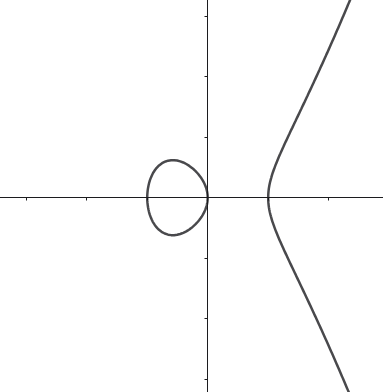
\includegraphics[width=0.25\linewidth]{Imagenes/Curva eliptica afin}
        	\caption{Curva algebraica afín $Z(y^2-x^3+x)$.}
        	\label{fig:curva-eliptica-afin}
        \end{figure}
        Ahora consideremos la homogeneización del polinomio $f(x,y)$ dada por
        \begin{equation*}
            F(X,Y,Z)=Z^3\left( \left(\frac{Y}{Z}\right)^2-\left(\frac{X}{Z}\right)^3+\frac{X}{Z}\right)=Y^2Z-X^3+XZ^2\in\cc[X,Y,Z].
        \end{equation*}
        Este polinomio es homogéneo de grado $3$ y su conjunto de ceros
        \begin{equation*}
            X=Z(F)=\{[X:Y:Z]\in\pp^2:F(X,Y,Z)=0\}
        \end{equation*}
        es una curva algebraica proyectiva. Ahora estudiemos sus puntos al infinito.\\
        Si $Z=0$, entonces $-X^3=0$. Esto implica que $X=0$. Por lo que el único punto al infinito es 
        \begin{equation*}
            [0:1:0].
        \end{equation*}
        Queremos ver ahora que $F$ no es singular en $[0:1:0]$. Las parciales de $F$ están dadas por
        \begin{equation*}
            F_X=-3X^2+Z^2,\qquad F_Y=2XZ,\qquad F_Z=Y^2+2XZ.
        \end{equation*}
        Con lo que, evaluando en el punto $[0:1:0]$, tenemos que
        \begin{equation*}
            F_X(0,1,0)=0,\qquad F_Y(0,1,0)=0,\qquad F_Z(0,1,0)=1.
        \end{equation*}
        Como no todas las parciales son cero, la curva es no singular en ese punto. Como $X$ es una curva proyectiva no singular, posee estructura natural de superficie de Riemann. Además, la fórmula de Plücker nos muestra que tiene género 1. (véase figura \ref{fig:toro}).
        
        Más aún, dado que $X\subset\pp^2$ entonces $X$ es una variedad compleja que vive dentro del plano proyectivo $\pp^2$. Más adelante veremos que, de hecho, es una subvariedad compleja y subvariedad analítica de $\pp^2$.
    \end{example}
    
    Considerando el caso de las variedades algebraicas proyectivas, surge de manera natural la siguiente pregunta: \textit{¿Qué variedades complejas pueden realizarse como subvariedades de algún espacio proyectivo complejo?} Tan sencilla como aparentemente específica, esta pregunta constituye la motivación central de este trabajo. Su respuesta, sin embargo, dista de ser inmediata y conduce a resultados considerablemente más profundos de lo que su formulación inicial pueda sugerir.
    
\section{Encaje Holomorfo}
	
	Antes de responder la pregunta anterior, introduciremos las nociones necesarias para formular con precisión el problema.
	
	Un \textit{encaje holomorfo} es una aplicación holomorfa que preserva la estructura compleja, la topología y la geometría exterior de una variedad compleja. El estudio de estos encajes nos revela profundas interacciones entre la geometría compleja, la teoría de haces y la cohomología, y nos conduce de manera natural a problemas centrales como la algebraización de variedades complejas y su relación con espacios proyectivos. En esta sección vamos A introducir el concepto de encaje holomorfo para analizar sus propiedades básicas, así como algunos ejemplos y contraejemplos relevantes.
	    
    \begin{definition}
        Sean $M$ y $N$ variedades complejas de dimensión $n$ y $k$ respectivamente. Una aplicación holomorfa $f:N\to M$ es un \textbf{encaje holomorfo} si satisface:
        \begin{enumerate}
            \item $f$ es inyectiva.
            \item (\textbf{Encaje topológico}) $f$ es un homeomorfismo con su imagen, es decir, $f:N\to f(N)$ es biyectiva, continua y con inversa continua ($f(N)$ lleva la topología del subespacio de $M$).
            \item Para cada $p\in N$, existen cartas $(U,\varphi)$ alrededor de $f(p)\in M$ y $(V,\psi)$ alrededor de $p\in N$ tales que $f(V)\subset U$ y en coordenadas
            \begin{equation*}
                \varphi\circ f\circ\psi^{-1}(z_1,\cdots,z_k)=(z_1,\cdots,z_k,0\cdots,0)\in\cc^n.
            \end{equation*}.
        \end{enumerate}
        Notemos que la condición $3$ nos indica que $f$, localmente, coincide con la inclusión $\cc^k\hookrightarrow\cc^n$, $z\mapsto (z,0)$.
    \end{definition}

    \begin{example}[Gráfica de una aplicación holomorfa]
    	Sea $N$ una variedad compleja de dimensión $n$ y $g:N\to\cc^{m}$ una aplicación holomorfa. Consideremos la aplicación
    	\begin{align*}
    		f:N\longrightarrow N\times\cc^{m}\\
    		z\mapsto(z,g(z)).
    	\end{align*}
    	Notemos que $f$ es una aplicación holomorfa pues cada una de sus componentes es holomorfa. Además, es inyectiva pues es la identidad en la primera entrada.\\
    	Luego, la aplicación inversa $f^{-1}:f(N)\to N$ está dada por
    	\begin{equation*}
    		f^{-1}(z,g(z))=z
    	\end{equation*}
    	la cual es continua. Por lo que $f:N\to f(N)$ es un homeomorfismo.\\ 
    	Consideremos una carta $(U,\varphi)$ una carta de $N$, $\varphi:U\to V\subset\cc^n$. Definamos la aplicación holomorfa $G:=g\circ \varphi^{-1}:V\to\cc^m$. De esta manera, obtenemos el biholomorfismo 
    	\begin{align*}
    		\Psi:V\times \cc^m\longrightarrow V\times \cc^m\\
    		(z,w)\mapsto (z,w-G(z)),
    	\end{align*}
    	pues su inversa es la aplicación $(z,w)\mapsto (z,w+G(z))$. Con lo cual, 
    	\begin{equation*}
    		\Psi(\varphi(U)\times\cc^m\cap f(U))=\{(z,0):z\in V\cap\varphi(U)\}=V\times\{0\}.
    	\end{equation*}
    	Definamos entonces la carta $\psi=\Psi\circ (\varphi\times \text{id})$ se cumple que
    	\begin{equation*}
    		\psi\circ f\circ \varphi^{-1}:V\to V\times\cc^m\subset \cc^{n+m} 
    	\end{equation*}
    	está dada por
    	\begin{equation*}
    		\psi\circ f\circ\varphi^{-1}(z)=(z,0)\in\cc^n\times\cc^m.
    	\end{equation*}
    	Por lo tanto, se cumple la definición de encaje holomorfo.\\
        Intuitivamente, $f$ está \enquote{dibujando} a la variedad $N$ dentro de $N\times\cc^m$ sin doblarla y sin autointersectarla.
        \begin{figure}[H]
        	\centering
        	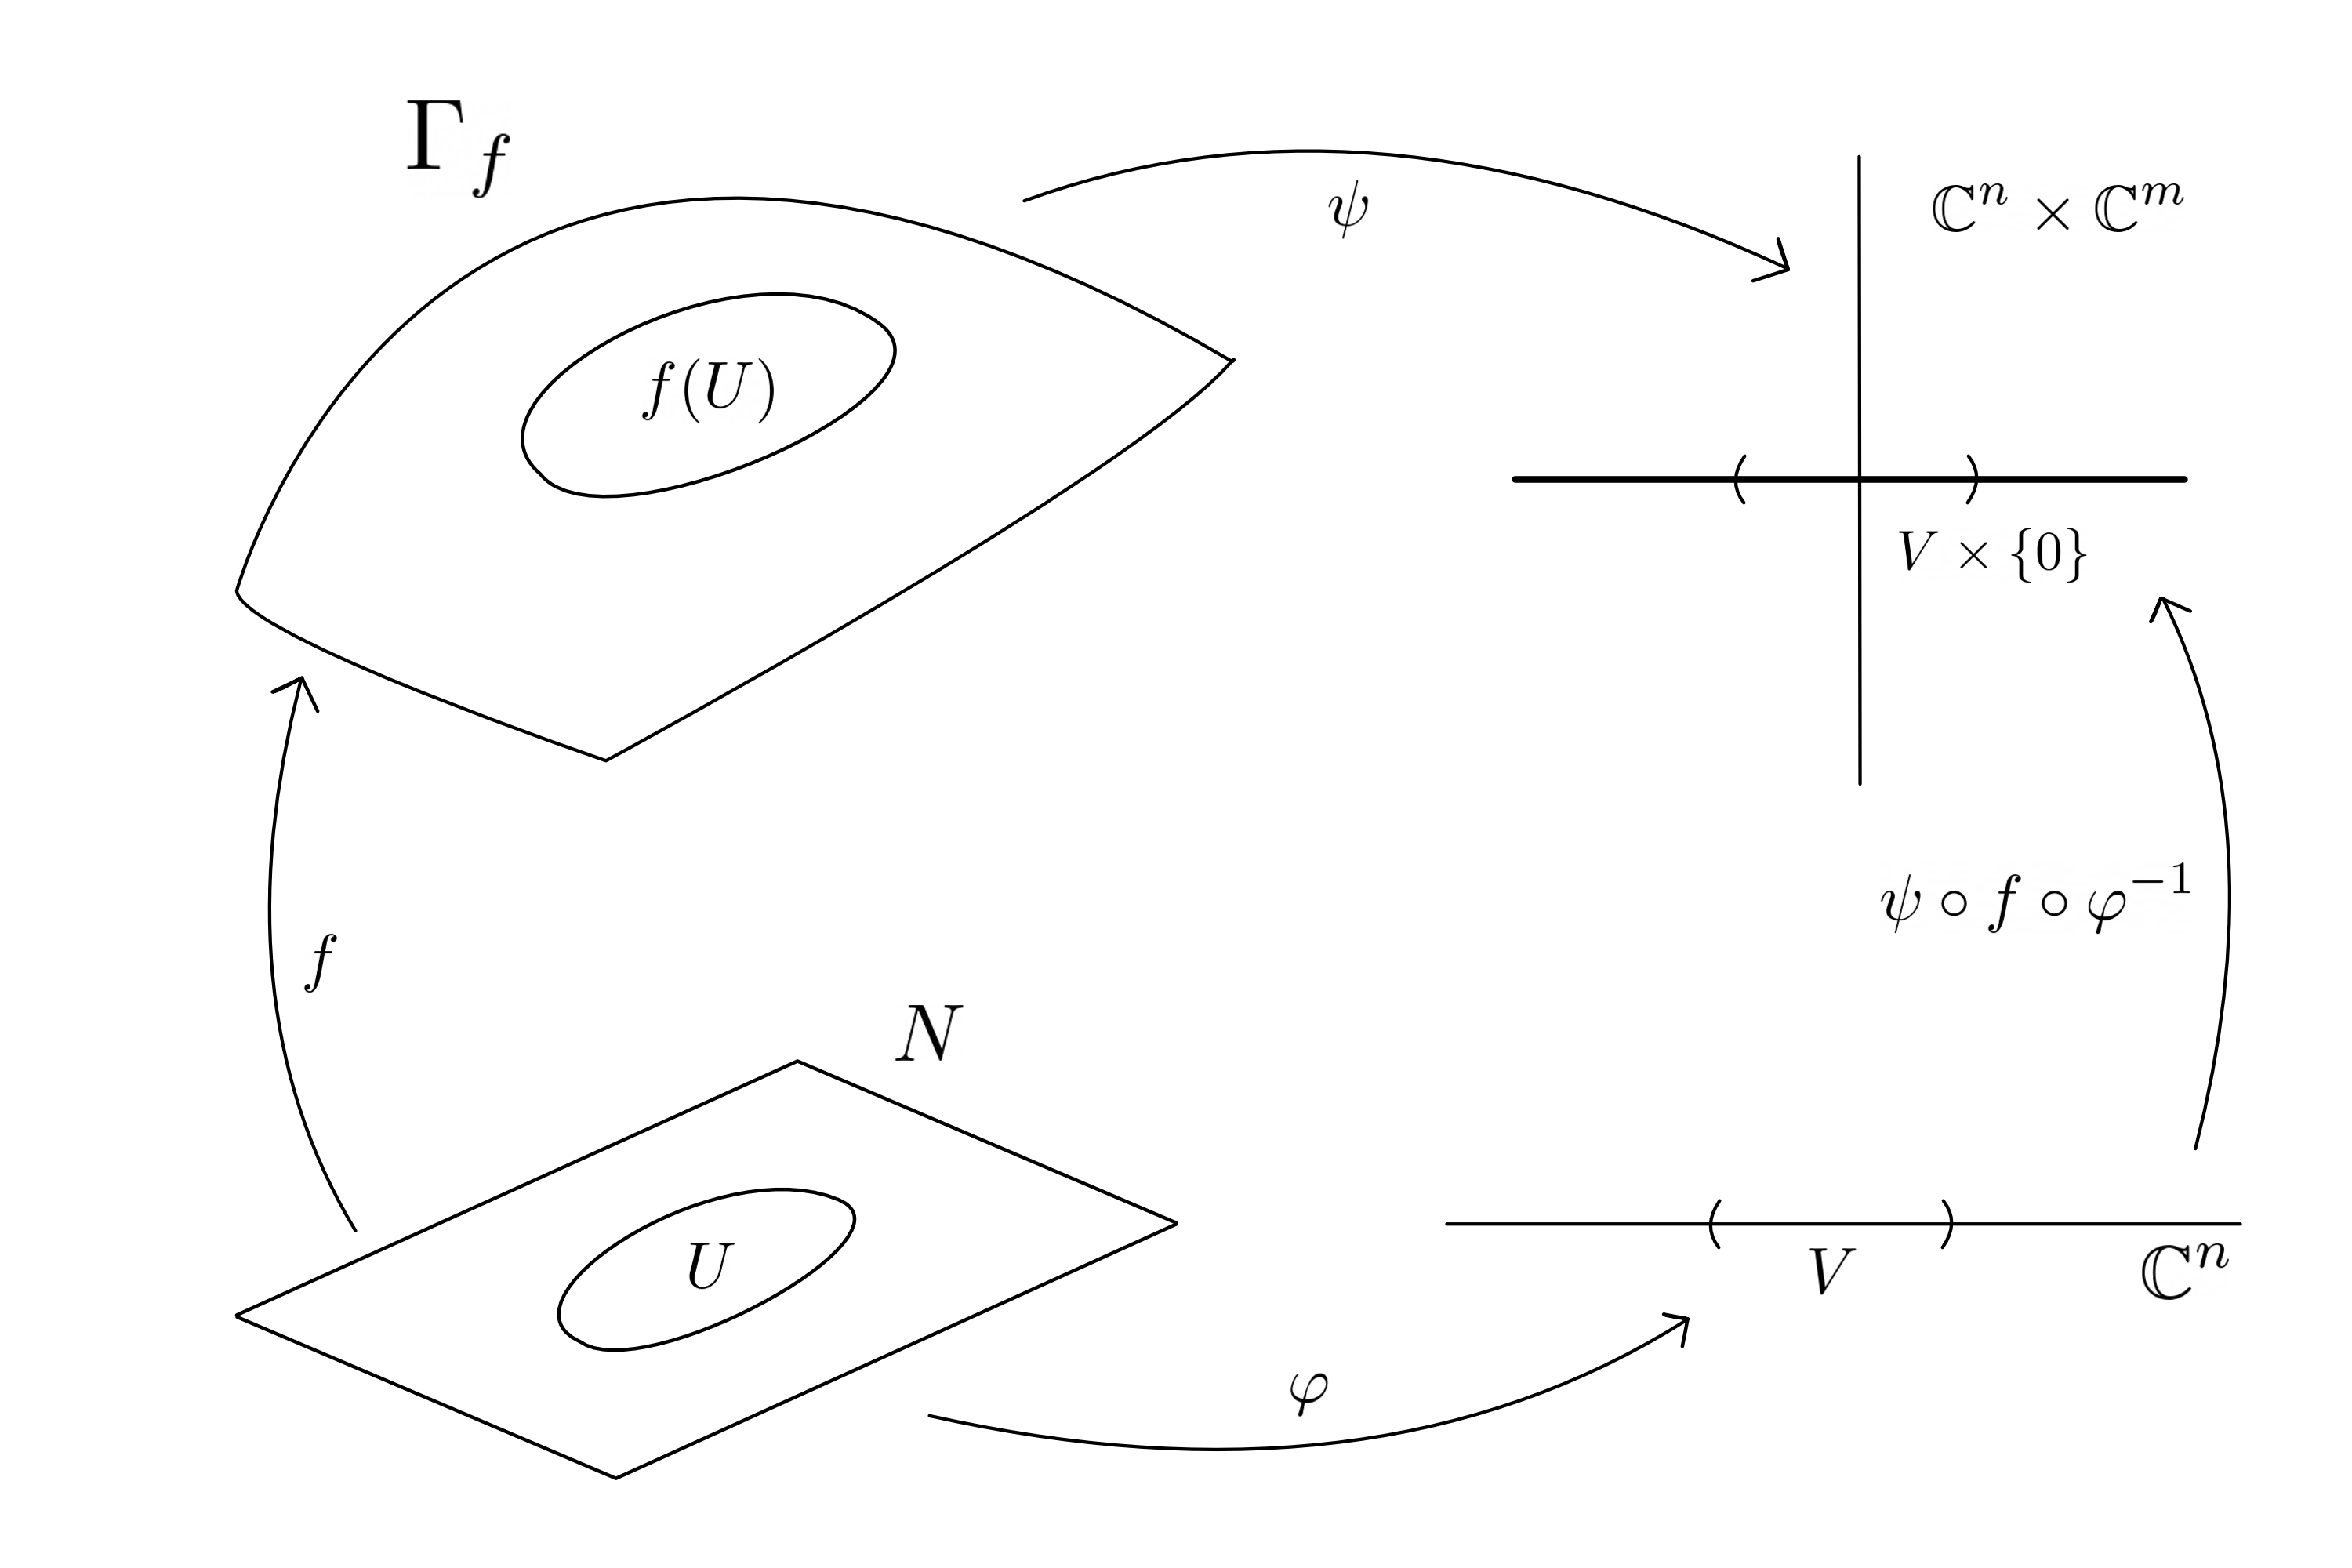
\includegraphics[width=0.6\linewidth]{Imagenes/Encaje de grafica}
        	\caption{Diagrama del encaje dada por una aplicación holomorfa.}
        	\label{fig:encaje-de-grafica}
        \end{figure}
         
    \end{example}
    
    
    \begin{definition}[Subvariedad compleja]
        Una variedad compleja $N$ es una subvariedad compleja (de dimensión $k$) de una variedad compleja $M$, con $\dim M=n$, si $N\subset M$ y existe un atlas holomorfo $\{U_i,\varphi_i\}$ de $M$ tal que 
        \begin{equation*}
            \varphi_i(U_i\cap N)\cong \varphi_i(U_i)\cap\cc^k
        \end{equation*}
        donde $\cc^k$ está encajado en $\cc^n$ por $z\mapsto (z,0)$. Definimos la \textbf{codimensión} de $N$ en $M$ como
        \begin{equation*}
            \mathrm{codim}N:=\dim M-\dim N=n-k.
        \end{equation*}
    \end{definition}
    
    \begin{remark}\label{subvariedadesporecuaciones} $ $
    	\begin{enumerate}
    		\item Si $N$ es una subvariedad compleja de $M$, entonces la inclusión $i:N\hookrightarrow M$ es un encaje holomorfo. Más aún, si $f:N\to M$ es un encaje holomorfo, entonces $f(N)$ es una subvariedad compleja de $M$.
    		\item Consideremos una variedad compleja $M$ y una subvariedad compleja $N\subset M$ de dimensión $k$. Por definición, para todo punto $p\in N$ existe una carta holomorfa $(U,\varphi)$ de $M$ tal que, después de identificar $\cc^k$ con el subespacio lineal
    		\begin{equation*}
    			\cc^k\times\{0\}\subset\cc^n
    		\end{equation*}
    		se cumple que
    		\begin{equation*}
    			\varphi(U\cap N)=\varphi(U)\cap (\cc^k\times \{0\}).
    		\end{equation*}
    		Si tomamos las coordenadas $z_1,\dots,z_n$ de $\cc^n$, entonces en dicha carta, $U\cap N$ queda descrita por las ecuaciones 
    		\begin{equation*}
    			z_{k+1}=\cdots=z_n=0.
    		\end{equation*}
    		Equivalentemente
    		\begin{equation*}
    			U\cap N=\bigcap_{j=k+1}^n f_j^{-1}(0)=Z(f_{k+1},\dots f_n),
    		\end{equation*}
    		donde $f_j=z_j\circ \varphi$. Por lo tanto, localmente $N$ es una subvariedad de intersección completa descrita por $n-k$ funciones holomorfas.
    	\end{enumerate}
    \end{remark}

	\begin{example}\label{algsonsubvariedades}
		Toda variedad algebraica no singular es una subvariedad compleja del espacio proyectivo. 
			Sea $V\subset\pp^n$ una variedad algebraica proyectiva no singular. Por definición, existe una cantidad finita de polinomios homogéneos $F_1,\dots,F_r\in \cc[x_0,\dots,x_n]$ tal que
			\begin{equation*}
				V=Z(F_1,\dots,F_r).
			\end{equation*}
			Fijemos una carta afín $U_i\subset \pp^n$
			y consideremos las coordenadas afines
			\begin{equation*}
				z_j=\frac{x_j}{x_i},\qquad j\neq i.
			\end{equation*}
			En esta carta, las ecuaciones homogéneas se transforman en ecuaciones polinómicas
			\begin{equation*}
				f_\ell(z_1,\dots,\widehat{z_i},\dots,z_n)=0,
				\qquad \ell=1,\dots,r,
			\end{equation*}
			donde cada $f_\ell$ es una función holomorfa sobre $U_i\cong \cc^n$. De esta manera,
			\begin{equation*}
				V\cap U_i=\{p\in U_i : f_1(p)=\cdots=f_r(p)=0\}
			\end{equation*}
			Sea $p\in V\cap U_i$. Como $V$ es no singular, el jacobiano de las ecuaciones tiene rango máximo igual a la codimensión de $V$ en $\pp^n$. Por el teorema de la función implícita \ref{funcionimplicita}, existen coordenadas holomorfas locales
			\begin{equation*}
				(w_1,\dots,w_n)
			\end{equation*}
			en una vecindad de $p$ tales que
			\begin{equation*}
			 V\cap U_i=Z(w_{k+1},\dots w_n).
			\end{equation*}
			Por lo observación \ref{subvariedadesporecuaciones}, $V$ es una subvariedad compleja de $\pp^n$, y la estructura compleja inducida coincide con la obtenida mediante las cartas holomorfas de $\pp^n$.
	\end{example}

	\begin{example}[Biholomorfismo que no es encaje]
		Sea $f:\cc\to\cc^*\times\cc^*$ la aplicación holomorfa
		\begin{equation*}
			f(z)=(e^z,e^{\alpha z}),
		\end{equation*}
		donde $\alpha\in\rr\setminus\mathbb{Q}$. Vamos a probar que $f$ es biholomorfa a su imagen. 
		
		Para la inyectividad, supongamos que $f(z)=f(w)$. Entonces
		\begin{equation*}
			e^{z-w}=1,\qquad e^{\alpha(z-w)}=1.
		\end{equation*}
		Así, existen $n,m\in \zz$ tales que
		\begin{equation*}
			z-w=2\pi i n,\qquad \alpha(z-w)=2\pi im.
		\end{equation*}
		Si $n\neq 0$, entonces $\alpha=m/n\in\mathbb{Q}$ lo cual es una contradicción. De esta manera, $n=0$ e implica que $z=w$. Por tanto, $f$ es inyectiva.
		
		Fijemos $z_0\in\cc$ y pongamos
		\begin{equation*}
			p=f(z_0).
		\end{equation*}
		Como la primera coordenada de $p=(p_1,p_2)$ es un punto en $\cc^*$, existe una vecindad $V$ de $p_1=e^{z_0}$ donde existe una rama del logaritmo
		\begin{equation*}
			\log_V:V\longrightarrow\cc.
		\end{equation*}
		Entonces, en una vecindad suficientemente pequeña de $p$ dentro de la imagen
		\begin{equation*}
			f^{-1}(w_1,w_2)=\log_V(w_1).
		\end{equation*}
		Con esto, $f^{-1}$ es holomorfa alrededor de cada punto de la imagen. Es decir, la aplicación
		\begin{equation*}
			f^{-1}:f(\cc)\longrightarrow\cc
		\end{equation*}
		es holomorfa. Con esto, $f$ es biholomorfa con su imagen. 
		
		Para probar que $f$ no es encaje, vamos a probar que $f:\cc\to f(\cc)$ no es un homeomorfismo si $f(\cc)$ lleva la topología del subespacio. 
		
		Consideremos la sucesión 
		\begin{equation*}
			z_n=2\pi in.
		\end{equation*} 
		Entonces
		\begin{equation*}
			f(z_n)=(1,e^{2\pi i\alpha n}).
		\end{equation*}
		Como $\alpha$ es irracional, la sucesión $\{e^{2\pi i\alpha n}\}$ es densa en $S^1$. Por lo que, existe una subsucesión $n_k$ tal que
		\begin{equation*}
			e^{2\pi i\alpha n_k}\longrightarrow 1.
		\end{equation*} 
		De esta manera, 
		\begin{equation*}
			f(z_{n_k})\longrightarrow (1,1)=f(0).
		\end{equation*}
		Sin embargo, $z_{n_k}=2\pi i n_k$ no converge a $0\in\cc$. Por lo que, la inversa $f^{-1}:f(\cc)\to\cc$ no es continua como espacios métricos, es decir, $f:\cc\to f(\cc)$ no es un homeomorfismo con la topología del subespacio de $f(\cc)$.
		\begin{figure}[H]
			\centering
			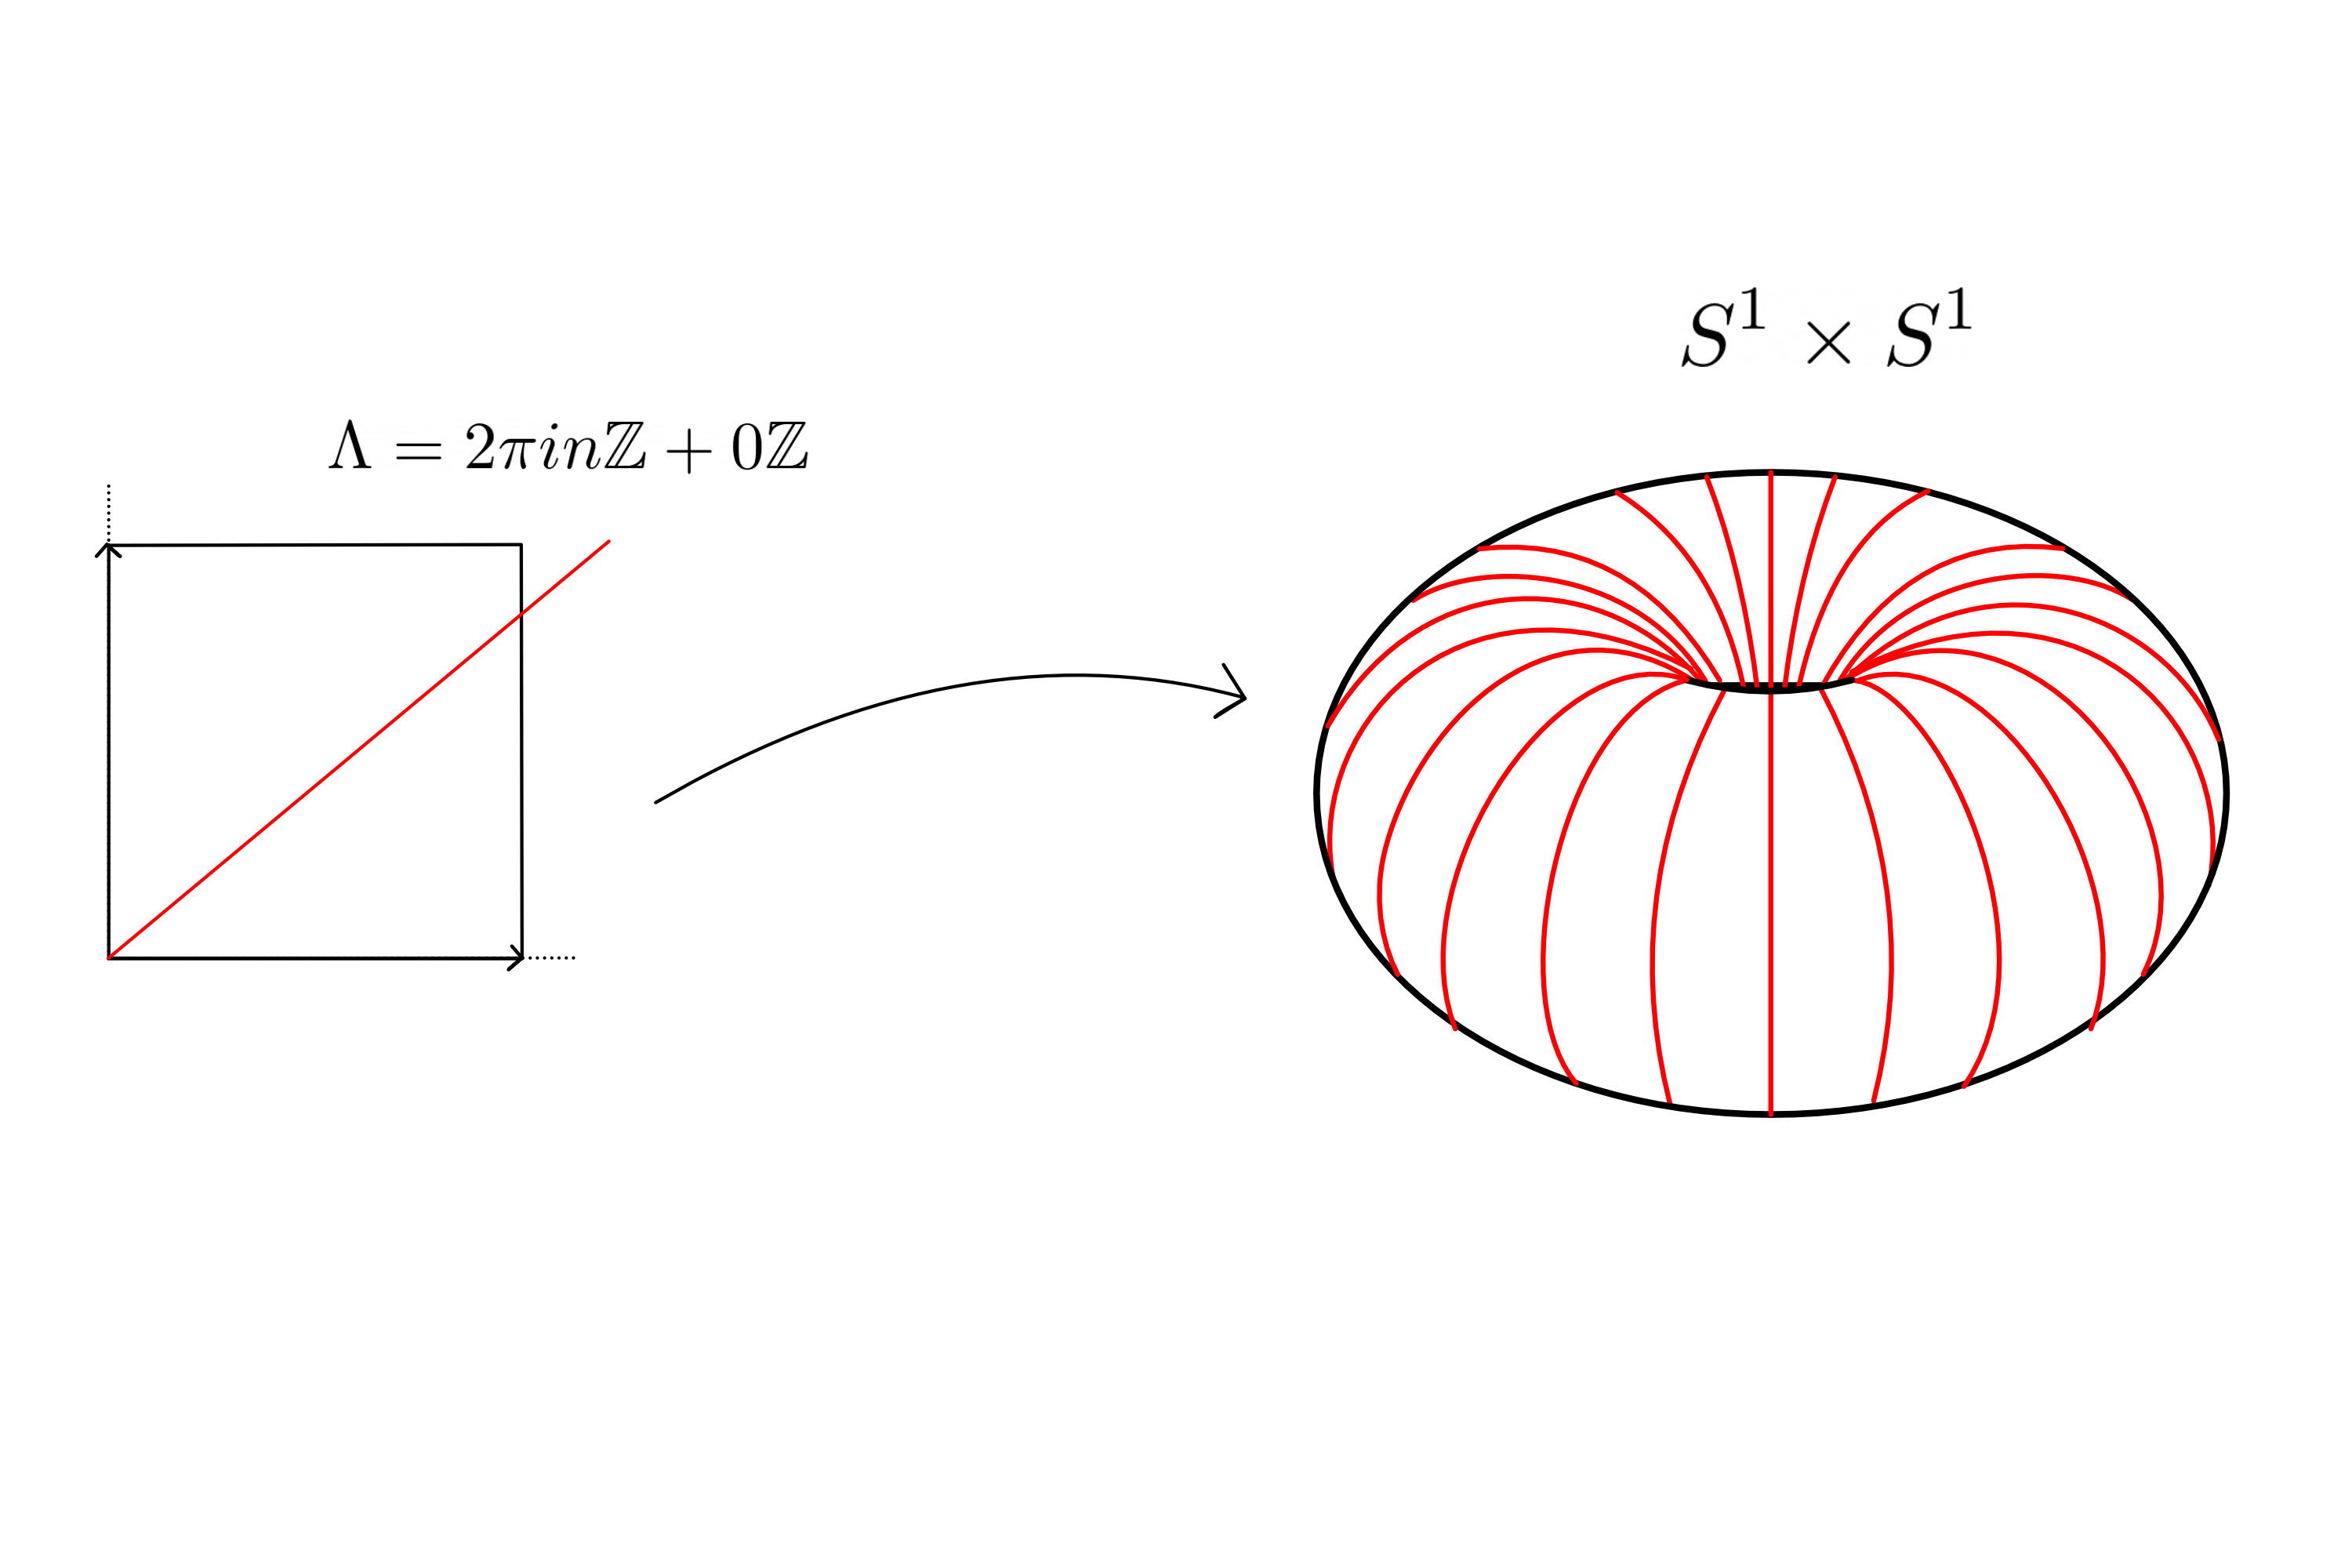
\includegraphics[width=0.7\linewidth]{Imagenes/biholomorfismo}
			\caption{Interpretación geométrica de la sucesión $z_n$.}
			\label{fig:biholomorfismo}
		\end{figure}
		
	\end{example}
	
    Como mencionabamos, el teorema de Whitney es un resultado general importante en la geometría diferencia real, pero no podemos tener un análogo directo en geometría compleja.
    
    \begin{example}\label{encajeccn}
        \textbf{No existen} subvariedades complejas compactas de $\cc^n$ de dimensión no cero. Ya que si $M\subset\cc^n$ es una subvariedad compleja compacta, entonces cada funcion de $\cc^n$ coordenada (proyección) $z_j$\footnote{Como $M$ es subvariedad, la inclusión $i:M\to \cc^n$ es holomorfa. Si $\pi_j:\cc^n\to\cc$ es la proyección a la $j$-ésima entrada, la función de $\cc^n$ coordenada $z_j=\pi_j\circ i:M\to \cc$ es una función holomorfa por ser composición de aplicaciones holomorfas.} restringida a $M$ es una función holomorfa global de $M$. Por el teorema \ref{holomorfasglobal}, $z_j$ es constante en cada componente conexa de $M$. Por lo que la inclusión $i:M\to\cc^n$ es constante en cada componente conexa de $M$. Con lo cual, cada componente conexa de $M$ consta de un único punto. Como $M$ es compacto, sólo puede tener un número finito de componentes conexas. En consecuencia, $M$ es un conjunto finito y, por tanto, tiene dimensión 0.
    \end{example}
    
    Ahora vamos a probar un resultado que nos ayudará a comprobar que una aplicación sea un encaje holomorfo. 
    
    \begin{propo}\label{encajesubvariedades}
    	Una aplicación holomorfa $f:M\to N$ es un encaje holomorfo si, y solo si, $f:M\to f(M)$ es un biholomorfismo y $f(M)\subset N$ es una subvariedad compleja.
    \end{propo}
    \begin{proof}
    		Primero, supongamos que $f:M\to N$ es un encaje. Por la condición de encaje topológico, $f:M\to f(M)$ es un homeomorfismo. En particular, la inversa $f^{-1}:f(M)\to M$ es continua.
    		
    		Tomemos $p\in M$ y sea $q=f(p)\in N$. Por la condición $(3)$ de encaje, existen cartas holomorfas $(V,\psi)$ alrededor de $q$ y $(U,\varphi)$ alrededor de $p$ tales que $f(U)\subset V$ y
    		\begin{equation*}
    			\psi\circ f\circ \varphi^{-1}(z_1,\dots,z_k)=(z_1,\dots,z_k,0,\dots,0)\in \cc^n.
    		\end{equation*}
    		Como $f$ es un homeomorfismo, $f(U)$ es abierto en $f(M)$ y $f(M)$ lleva la topología de subespacio, al reducir $V$ si es necesario podemos suponer que $V\cap f(M)=f(U)$. Entonces, en este abierto la inversa de $f$ se escribe en coordenadas como la proyección sobre las primeras $k$ coordenadas:
    		\begin{equation*}
    			\varphi\circ f^{-1}\circ \psi^{-1}(w_1,\dots,w_n)=(w_1,\dots,w_k),
    			\qquad (w_1,\dots,w_n)\in \psi(V\cap f(M)).
    		\end{equation*}
    		Esta expresión es holomorfa. Como $p$ era arbitrario, $f^{-1}$ es holomorfa en todo $f(M)$. Por tanto, $f:M\to f(M)$ es un biholomorfismo.
    		
    		Para ver que $f(M)$ es una subvariedad compleja de $N$, observemos que las mismas cartas satisfacen
    		\begin{equation*}
    			\psi(V\cap f(M))=\psi(V)\cap (\cc^k\times \{0\}).
    		\end{equation*}
  			Es decir, $f(M)$ es una subvariedad compleja de $N$.
  			
  			Ahora, supongamos que $f:M\to f(M)$ es un biholomorfismo y $f(M)$ es subvariedad compleja. Entonces es inmediato que $f:M\to f(M)$ es un encaje topológico donde $f(M)$ lleva la topología del subespacio. 
  			
  			Sea $p\in M$ y $q=f(p)\in N$. Como $f(M)$ es una subvariedad compleja, existe una carta holomorfa $(V,\psi)$ de $q$ tal que
  			\begin{equation*}
  				\psi(V\cap f(M))=\psi(V)\cap (\cc^k\times \{0\}).
  			\end{equation*} 
  			Sea $U:=f^{-1}(V)\subset M$. Entonces $f|_U:U\to V\cap f(M)$ sigue siendo un biholomorfismo. Consideremos la proyección a las primeras $k$ entradas
  			\begin{align*}
  				&\pi:\cc^n\longrightarrow \cc^k\\
  				(z_1,\dots,z_k&,\dots,z_n)\mapsto (z_1,\dots, z_k).
  			\end{align*} 
  			Definamos entonces 
  			\begin{equation*}
  				\varphi:=\pi\circ \psi\circ f|_U:U\longrightarrow\cc^k.
  			\end{equation*}
    		Como $\psi(f(V))\subset \cc^k\times \{0\}$, la aplicación restringida a $\pi$ sigue siendo un biholomorfismo sobre $\cc^k$. Por lo que, $\varphi$ es una carta holomorfa alrededor de $p$.
    		
    		Además, para todo $z\in\varphi(U)\subset\cc^k$, 
    		\begin{equation*}
    			\psi\circ f\circ \varphi^{-1}(z)=(z,0)\in\cc^n.
    		\end{equation*}
    		Por lo tanto, $f$ satisface la propiedad $(3)$ y concluimos que $f$ es un encaje holomorfo. 
    \end{proof}
    
    Un biholomorfismo sobre su imagen solo exige que existe una inversa holomorfa entre conjuntos, pero no garantiza que el dominio tenga la estructura analítica de la subvariedad imagen. En otras palabras, un encaje holomorfo es un biholomorfismo sobre su imagen cuya imagen es una subvariedad compleja. 
    
%    \begin{example}
%        Consideremos la aplicación holomorfa $f:\cc\to\pp^1$ dada por 
%        \begin{equation*}
%        	f(z)=[z:1]
%        \end{equation*}
%      	Notemos que $f$ es un homeomorfismo pues es la inversa de una carta afín de $\pp^1$. Así, determina un biholomorfismo entre $\cc$ y $\pp^1\setminus \{[1:0]\}$. Sin embargo, $\pp^1\setminus\{[1:0]\}$ no es una subvariedad compleja de $\pp^1$. Por lo tanto, $f$ no es un encaje holomorfo.
%      	\begin{figure}[H]
%      		\centering
%      		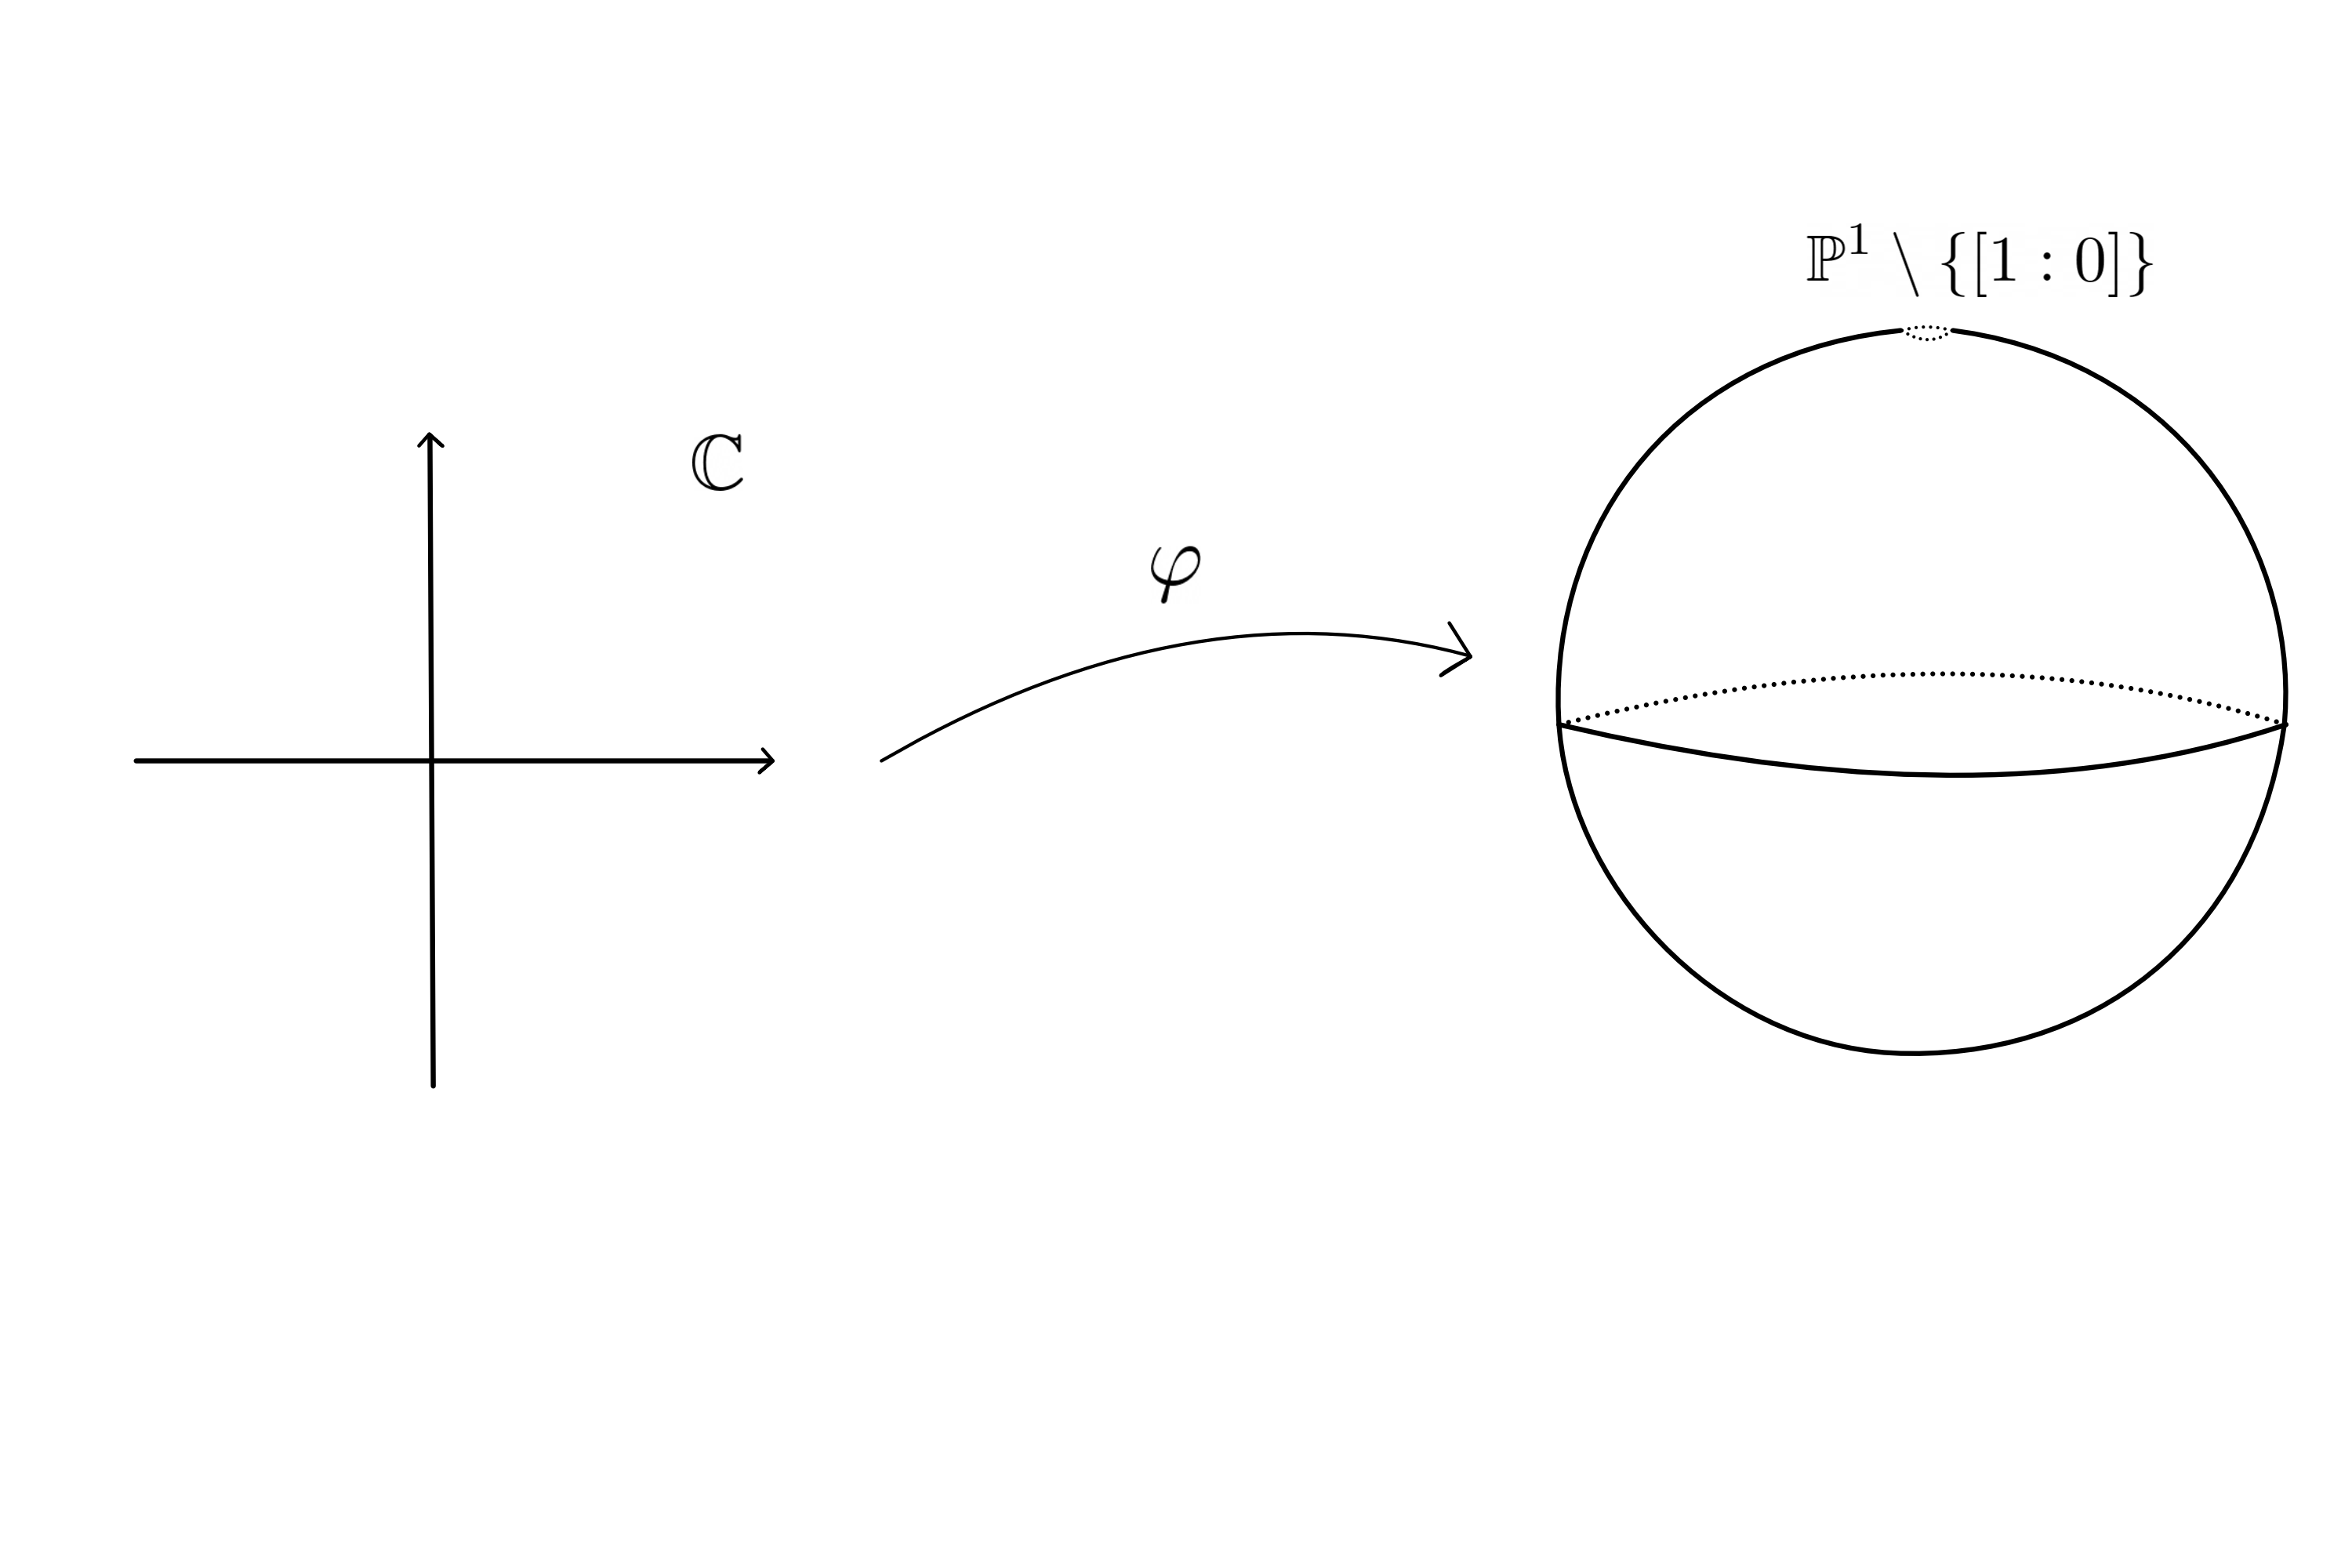
\includegraphics[width=0.5\linewidth]{Imagenes/no encaje a P1}
%      		\caption{Inmersión de $\cc$ en $\pp^1$.}
%      		\label{fig:no-encaje-a-p1}
%      	\end{figure}
%      	
%    \end{example}
   	
   	Un encaje puede entenderse, en este contexto, como una manera de \enquote{incrustar} una variedad en otra sin perder su estructura compleja. En particular, nos interesan los encajes en espacios proyectivos, cuya importancia será gracias al teorema de Chow, que abordaremos en el siguiente capítulo. Finalmente, introduzcamos la noción de una variedad que admita un encaje al espacio proyectivo.
   	
   	\begin{definition}
   		Una variedad compleja $M$ se dice \textbf{proyectiva} si admite un biholomorfismo sobre una subvariedad compleja de algún espacio proyectivo complejo.
   	\end{definition}
   	
   	\subsection{El caso de las curvas complejas}
   	
   	El problema del encaje proyectivo ya está completamente resuelto en dimensión uno. La construcción de dicho encaje constituye el antecedente directo a todo nuestro desarrollo y se basa en la teoría de divisores y el teorema de \textit{Riemann-Roch}.
   	
   	Consideremos una superficie de Riemann compacta $S$ de género $g$. Recordemos que un \textbf{divisor} sobre $S$ es una función $D:S\to \zz$ con soporte finito. Se suele escribir como una suma formal
   	\begin{equation*}
   		D=\sum_{p\in S} n_p\cdot p
   	\end{equation*}
   	donde $D(p)=n_p$ y este número es llamado \textbf{peso} de $p$.
   	
   	Por esta manera, podemos definir el \textbf{grado} del divisor $D$ como el valor finito.
   	\begin{equation*}
   		\deg(D)=\sum_{p\in S} n_p
   	\end{equation*}
   	Dado un divisor $D$, podemos considerar el \textbf{espacio de funciones meromorfas asociado al divisor} dado por el conjunto
   	\begin{equation*}
   		L(D):=\{f\in\mathscr{M}(S):\mathrm{ord}_{p}f\geq -n_p\text{ para todo }p\in S\}.
   	\end{equation*}
   	Este espacio es un $\cc$-espacio vectorial finito y su dimensión se denota como $\ell(D):=\dim_{\cc}L(D)$.\\
   	Vamos a construir una aplicación holomorfa con esta información. Consideremos $\{s_1,\cdots, s_{\ell(D)}\}$ una base del espacio $L(D)$. Sea $p\in S$, $(U,z)$ una carta alrededor de $p$ tal que $z(p)=0$ y
   	\begin{equation*}
   		k=\min_j\{\mathrm{ord}_ps_j\}.
   	\end{equation*}
   	Así, podemos escribir a $s_j$ como
   	\begin{equation*}
   		s_j=z^kg_j,
   	\end{equation*}
   	donde $g_j\in\oo_S(U)$. De esta manera, al menos una de las funciones $g_j$ no se anula en $p$, por lo que el vector
   	\begin{equation*}
   		(g_1(p),\dots,g_{\ell(D)}(p))
   	\end{equation*}
   	es no nulo y determina un punto en $\pp^{\ell(D)-1}$. Además, la definición es independiente de la carta. Con lo cual, la aplicación
   	\begin{align*}
   		\varphi_D:S\longrightarrow \pp^{\ell(D)-1}\\
   		p\mapsto[g_1(p):\cdots:g_{\ell(D)}(p)].
   	\end{align*}
   	está bien definida.
   	
   	\begin{theorem}\label{encajedesuperficies}
   		Sea $S$ una superficie de Riemann compacta de género $g$. Consideremos $D$ un divisor sobre $S$ tal que $\deg(D)\geq 2g+1$, entonces la aplicación
   		\begin{equation*}
   			\varphi_D:S\longrightarrow \pp^{\ell(D)-1}
   		\end{equation*}
   		es un encaje holomorfo.
   	\end{theorem}
   	Una demostración puede consultarse en \parencite[Teo.~5.111]{zaldrimann}. En consecuencia, toda superficie de Riemann compacta es proyectiva.
	
	Nuestro objetivo será extender esta construcción a variedades complejas de dimensión arbitraria mediante haces lineales y estudiar bajo qué hipótesis es posible obtener un encaje proyectivo.
	
\section{Haces Lineales holomorfos}

%	Un \textit{haz lineal} puede entenderse como una familia de rectas complejas parametrizadas por una variedad compleja. A cada punto $p\in M$ se le asocia un espacio vectorial complejo de dimensión uno, llamado fibra, de manera que todas estas fibras se \enquote{ensamblan} holomórficamente formando una nueva variedad $L$, denominada espacio total. Localmente, este espacio se comporta como un producto $U\times$, aunque globalmente puede presentar una geometría mucho más rica.
	
    Un \textit{haz lineal} es un objeto geométrico que asocia, a cada punto de una variedad $M$, un espacio vectorial de dimensión uno, de modo que todos estos espacios se \enquote{ensamblan} suavemente formando un nuevo espacio. Este espacio total se proyecta sobre $M$ y, cerca de cualquier punto, se ve exactamente como un producto entre un abierto y $\cc$. Así, el haz lineal puede imaginarse como una variedad \enquote{engrosada} por fibras lineales que se extienden continuamente por encima de $M$ en cada punto.

    \begin{definition}
	Sea $M$ una variedad compleja. Un \textbf{haz lineal} (holomorfo) es una triada $ (L,\pi, M) $ con la siguiente información:
	\begin{itemize}
		\item $L$ es una variedad compleja y $\pi:L\to M$ es una aplicación holomorfa sobreyectiva.
		\item Para cada punto $ p\in M $, la fibra $L_p:=\pi^{-1}(p)$ es homeomorfa a un $\cc$-espacio vectorial de dimensión $1$. Esto es, $L_p\cong \cc$. 
		\item Existe una cubierta de $\{U_i\}_{i\in I}$ de $M$ y biholomorfismos 
		\begin{align*}
			\phi_i:\pi^{-1}(U_i)\to U_i\times\cc,
		\end{align*}
		llamados \textbf{trivialización local}, tales que el siguiente diagrama conmuta
		\begin{center}
			\begin{tikzcd}
				{L|_{U_i}:=\pi^{-1}(U_i)} && {U_i\times\cc} \\
				\\
				& M
				\arrow["{\phi_i}", from=1-1, to=1-3]
				\arrow["\pi"', from=1-1, to=3-2]
				\arrow["{pr_1}", from=1-3, to=3-2]
			\end{tikzcd}
		\end{center}
		y si $ p\in U_i$, entonces la restricción a las fibras es un morfismo de $ \cc $-espacios vectoriales
		\begin{center}
			\begin{tikzcd}
				{L_p=\pi^{-1}(p)} && {\{p\}\times \cc\subset U_i\times\cc} && {\cc}
				\arrow["\phi_i|_{L_p}", from=1-1, to=1-3]
				\arrow["{\pi_2}", from=1-3, to=1-5]
			\end{tikzcd}
		\end{center}
		
		\begin{figure}[H]
			\centering
			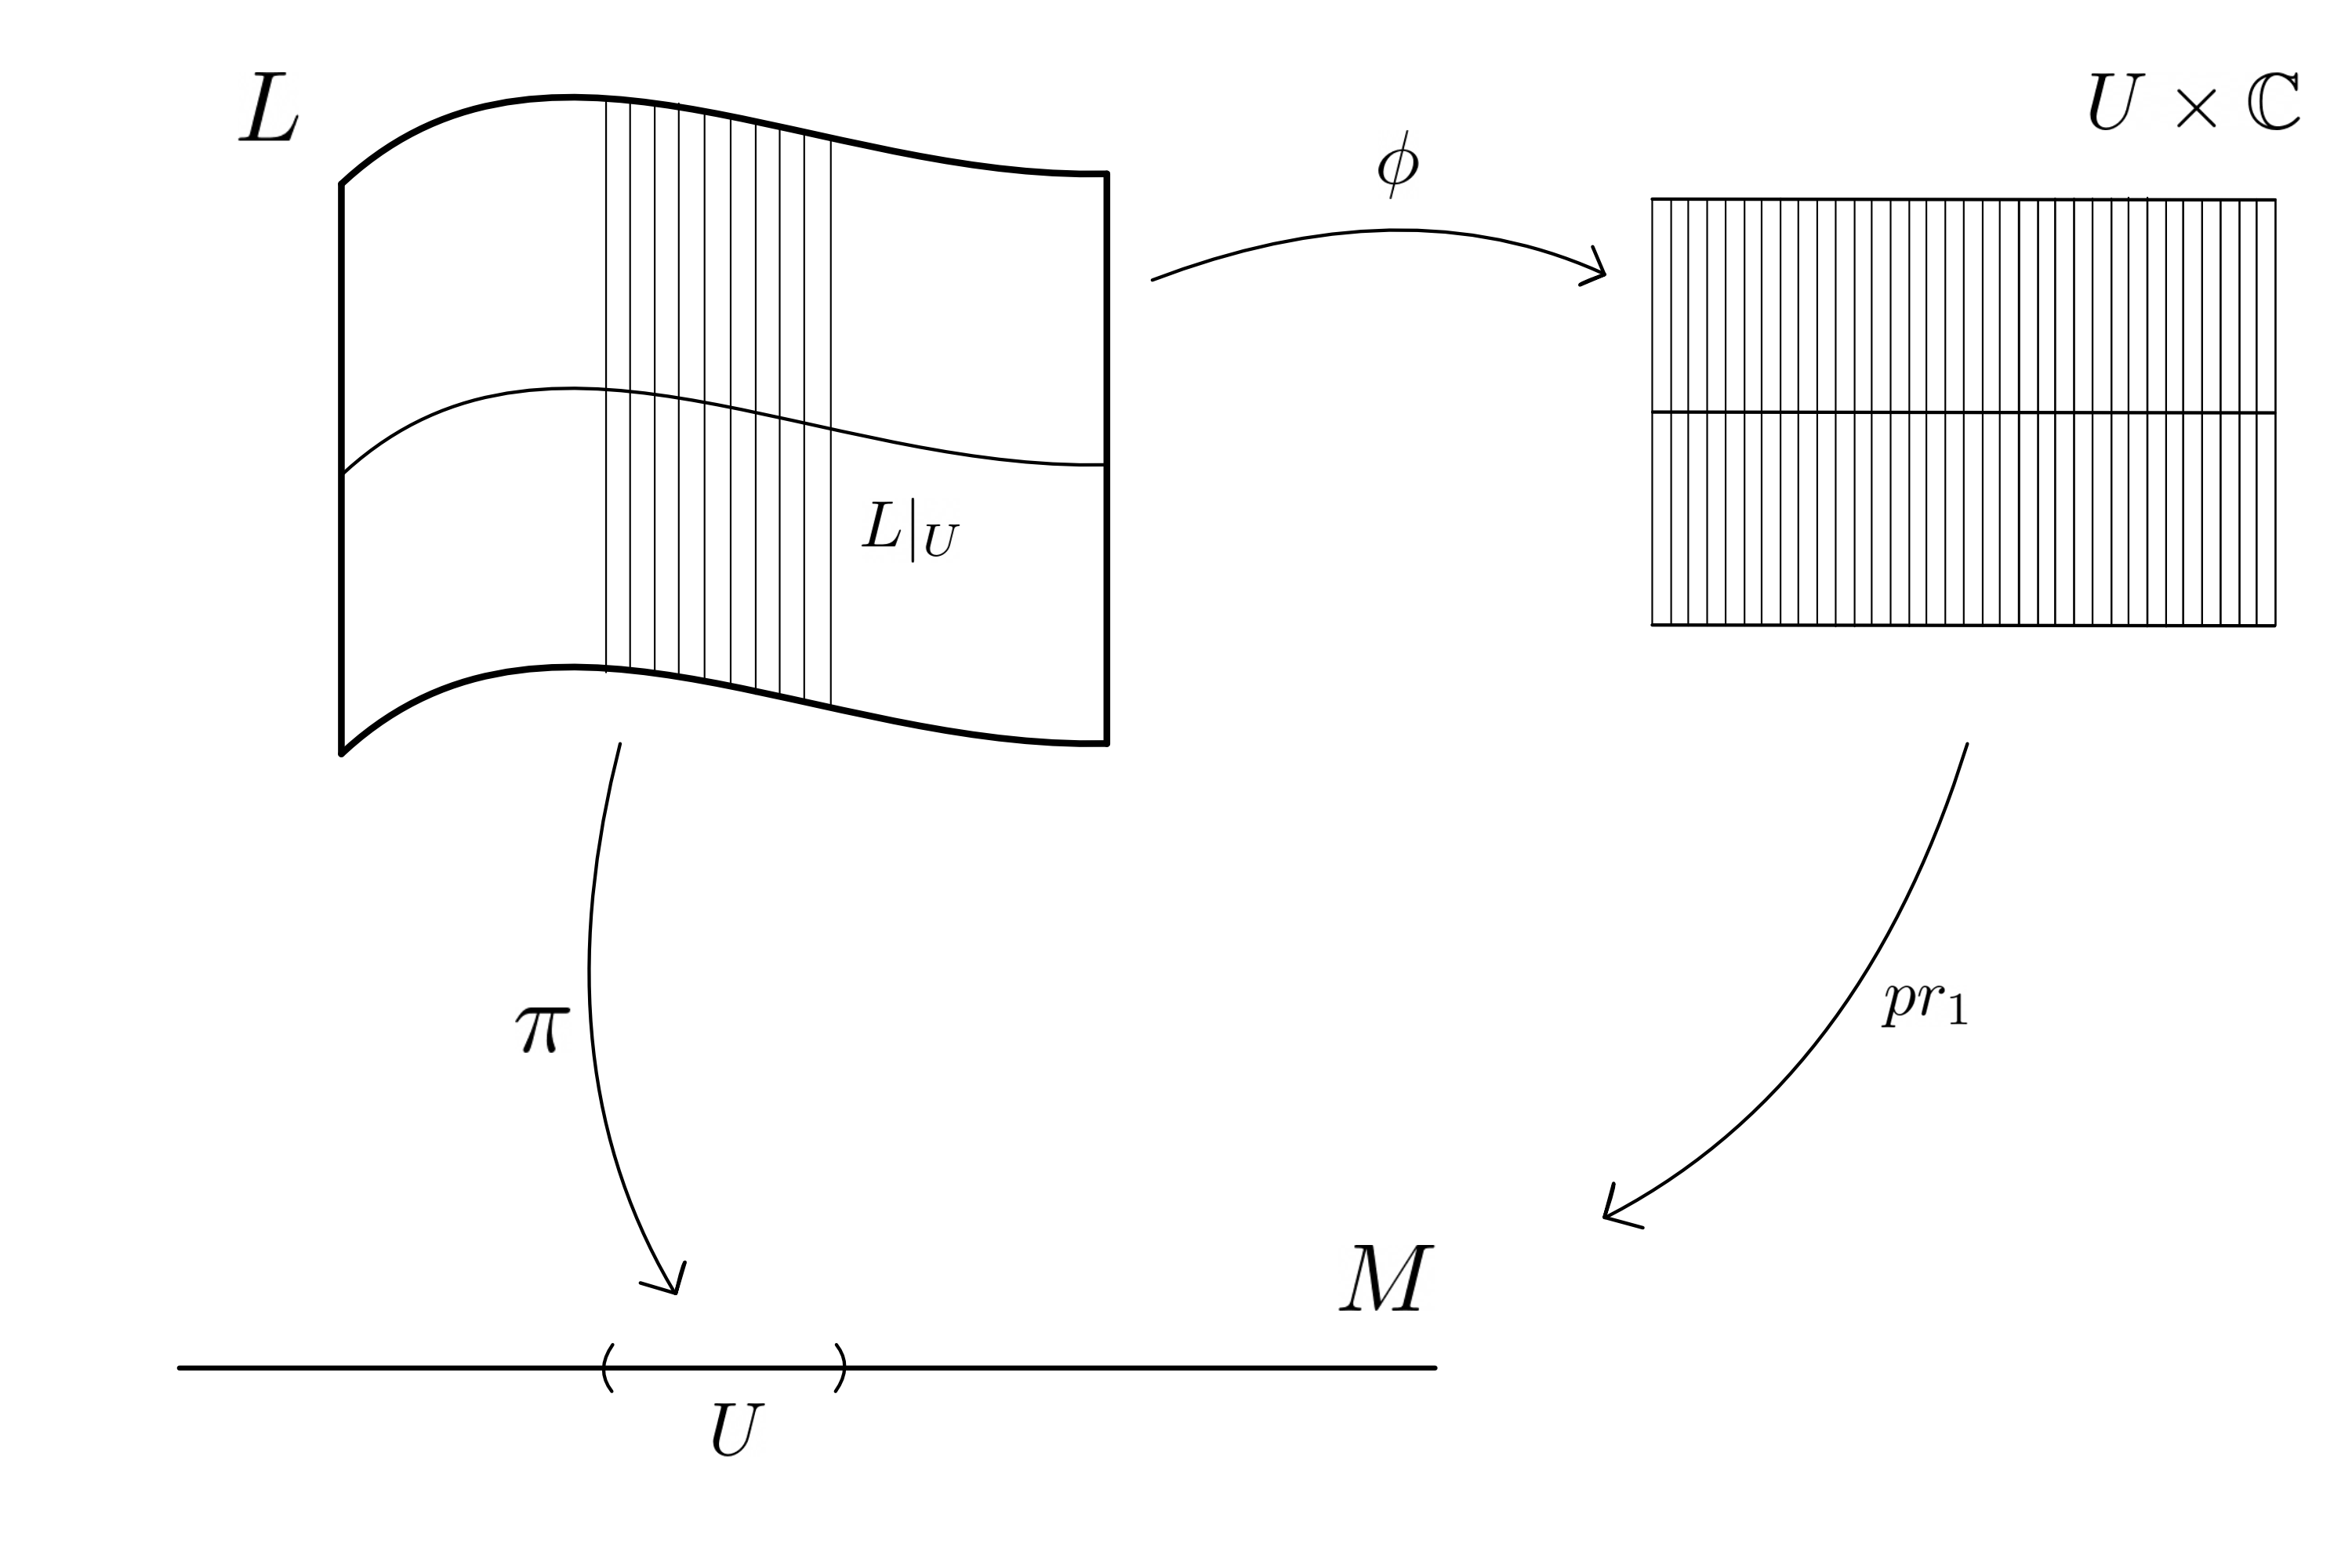
\includegraphics[width=0.7\linewidth]{Imagenes/definicion de haz}
			\caption{Una trivialización de un haz lineal.}
			\label{fig:definicion-de-haz}
		\end{figure}
		
	\end{itemize}
    \end{definition}

    \begin{remark}
    	Sea $ (L,\pi, M) $ es un haz lineal holomorfo. Al espacio $M$ se le llama \textbf{espacio base}, al espacio $ L $ se le llama \textbf{espacio total} y a la función sobreyectiva $\pi:L\to M$ se le llama \textbf{proyección}. Cuando la proyección es clara, se suele denotar $ L\longrightarrow M$ o
    	\begin{center}
    		\begin{tikzcd}
    			L \\
    			\\
    			M
    			\arrow[no head, from=1-1, to=3-1]
    		\end{tikzcd}
    	\end{center}
    	Y si el espacio base también es claro o es fijo, solo decimos que $L$ es un haz lineal. 
    \end{remark}

    \begin{example}[Haz trivial]\label{haztrivial}
    	Sea $M$ un espacio topológico. Notemos que el espacio producto $L:=M\times\cc$ tiene una función proyección a la primera entrada
    	\begin{align*}
    		\pi:&M\times\cc\longrightarrow M\\
    		&(p,z)\mapsto p
    	\end{align*}
    	la cual es holomorfa y sobreyectiva. Si $p\in M$, entonces
    	\begin{align*}
    		L_p=\pi^{-1}(p)=\{p\}\times\cc\cong \cc.
    	\end{align*}
    	Luego, para toda cubierta $\{U_i\}_{i\in I}$ de $M$, tenemos que 
    	\begin{align*}
    		L|_{U_i}=\pi^{-1}(U_i)=U_i\times \cc.
    	\end{align*} 
    	Así, la trivialización local está dada por $\{U_i\}_{i\in I}$ y los biholomorfismos identidad $id_i:L|_{U_i}\to U_i\times\cc$ y claramente conmuta el diagrama
    	\begin{center}
    		\begin{tikzcd}
    			{L|_{U_i}:=\pi^{-1}(U_i)} && {U_i\times\cc} \\
    			\\
    			& M
    			\arrow["{id_i}", from=1-1, to=1-3]
    			\arrow["\pi"', from=1-1, to=3-2]
    			\arrow["{\pi_1}", from=1-3, to=3-2]
    		\end{tikzcd}
    	\end{center}
    	Por lo tanto, $(M\times\cc,\pi_1,M)$ es un haz lineal sobre $M$. 
    \end{example}
    
    Sea $L$ un haz lineal sobre la variedad compleja $M$. Tomemos una trivialización ${U_i}*{i\in I}$ de $L$. Es decir, para cada $i$ existe un biholomorfismo
    \begin{equation*}
    	\psi_i :L|_{U_i}\longrightarrow U_i\times \mathbb{C}
    \end{equation*}
    En una intersección $U_{ij}:=U_i\cap U_j$, ambas trivializaciones difieren por multiplicación por una función holomorfa no nula
    \begin{equation*}
    	\psi_i\circ \psi_j^{-1}(x,z)=(x,g_{ij}(x)z),
    	\qquad x\in U_i\cap U_j,
    \end{equation*}
    donde
    \begin{equation*}
    	g_{ij}\in \mathcal{O}^*(U_i\cap U_j).
    \end{equation*}
    
    \begin{figure}[H]
    	\centering
    	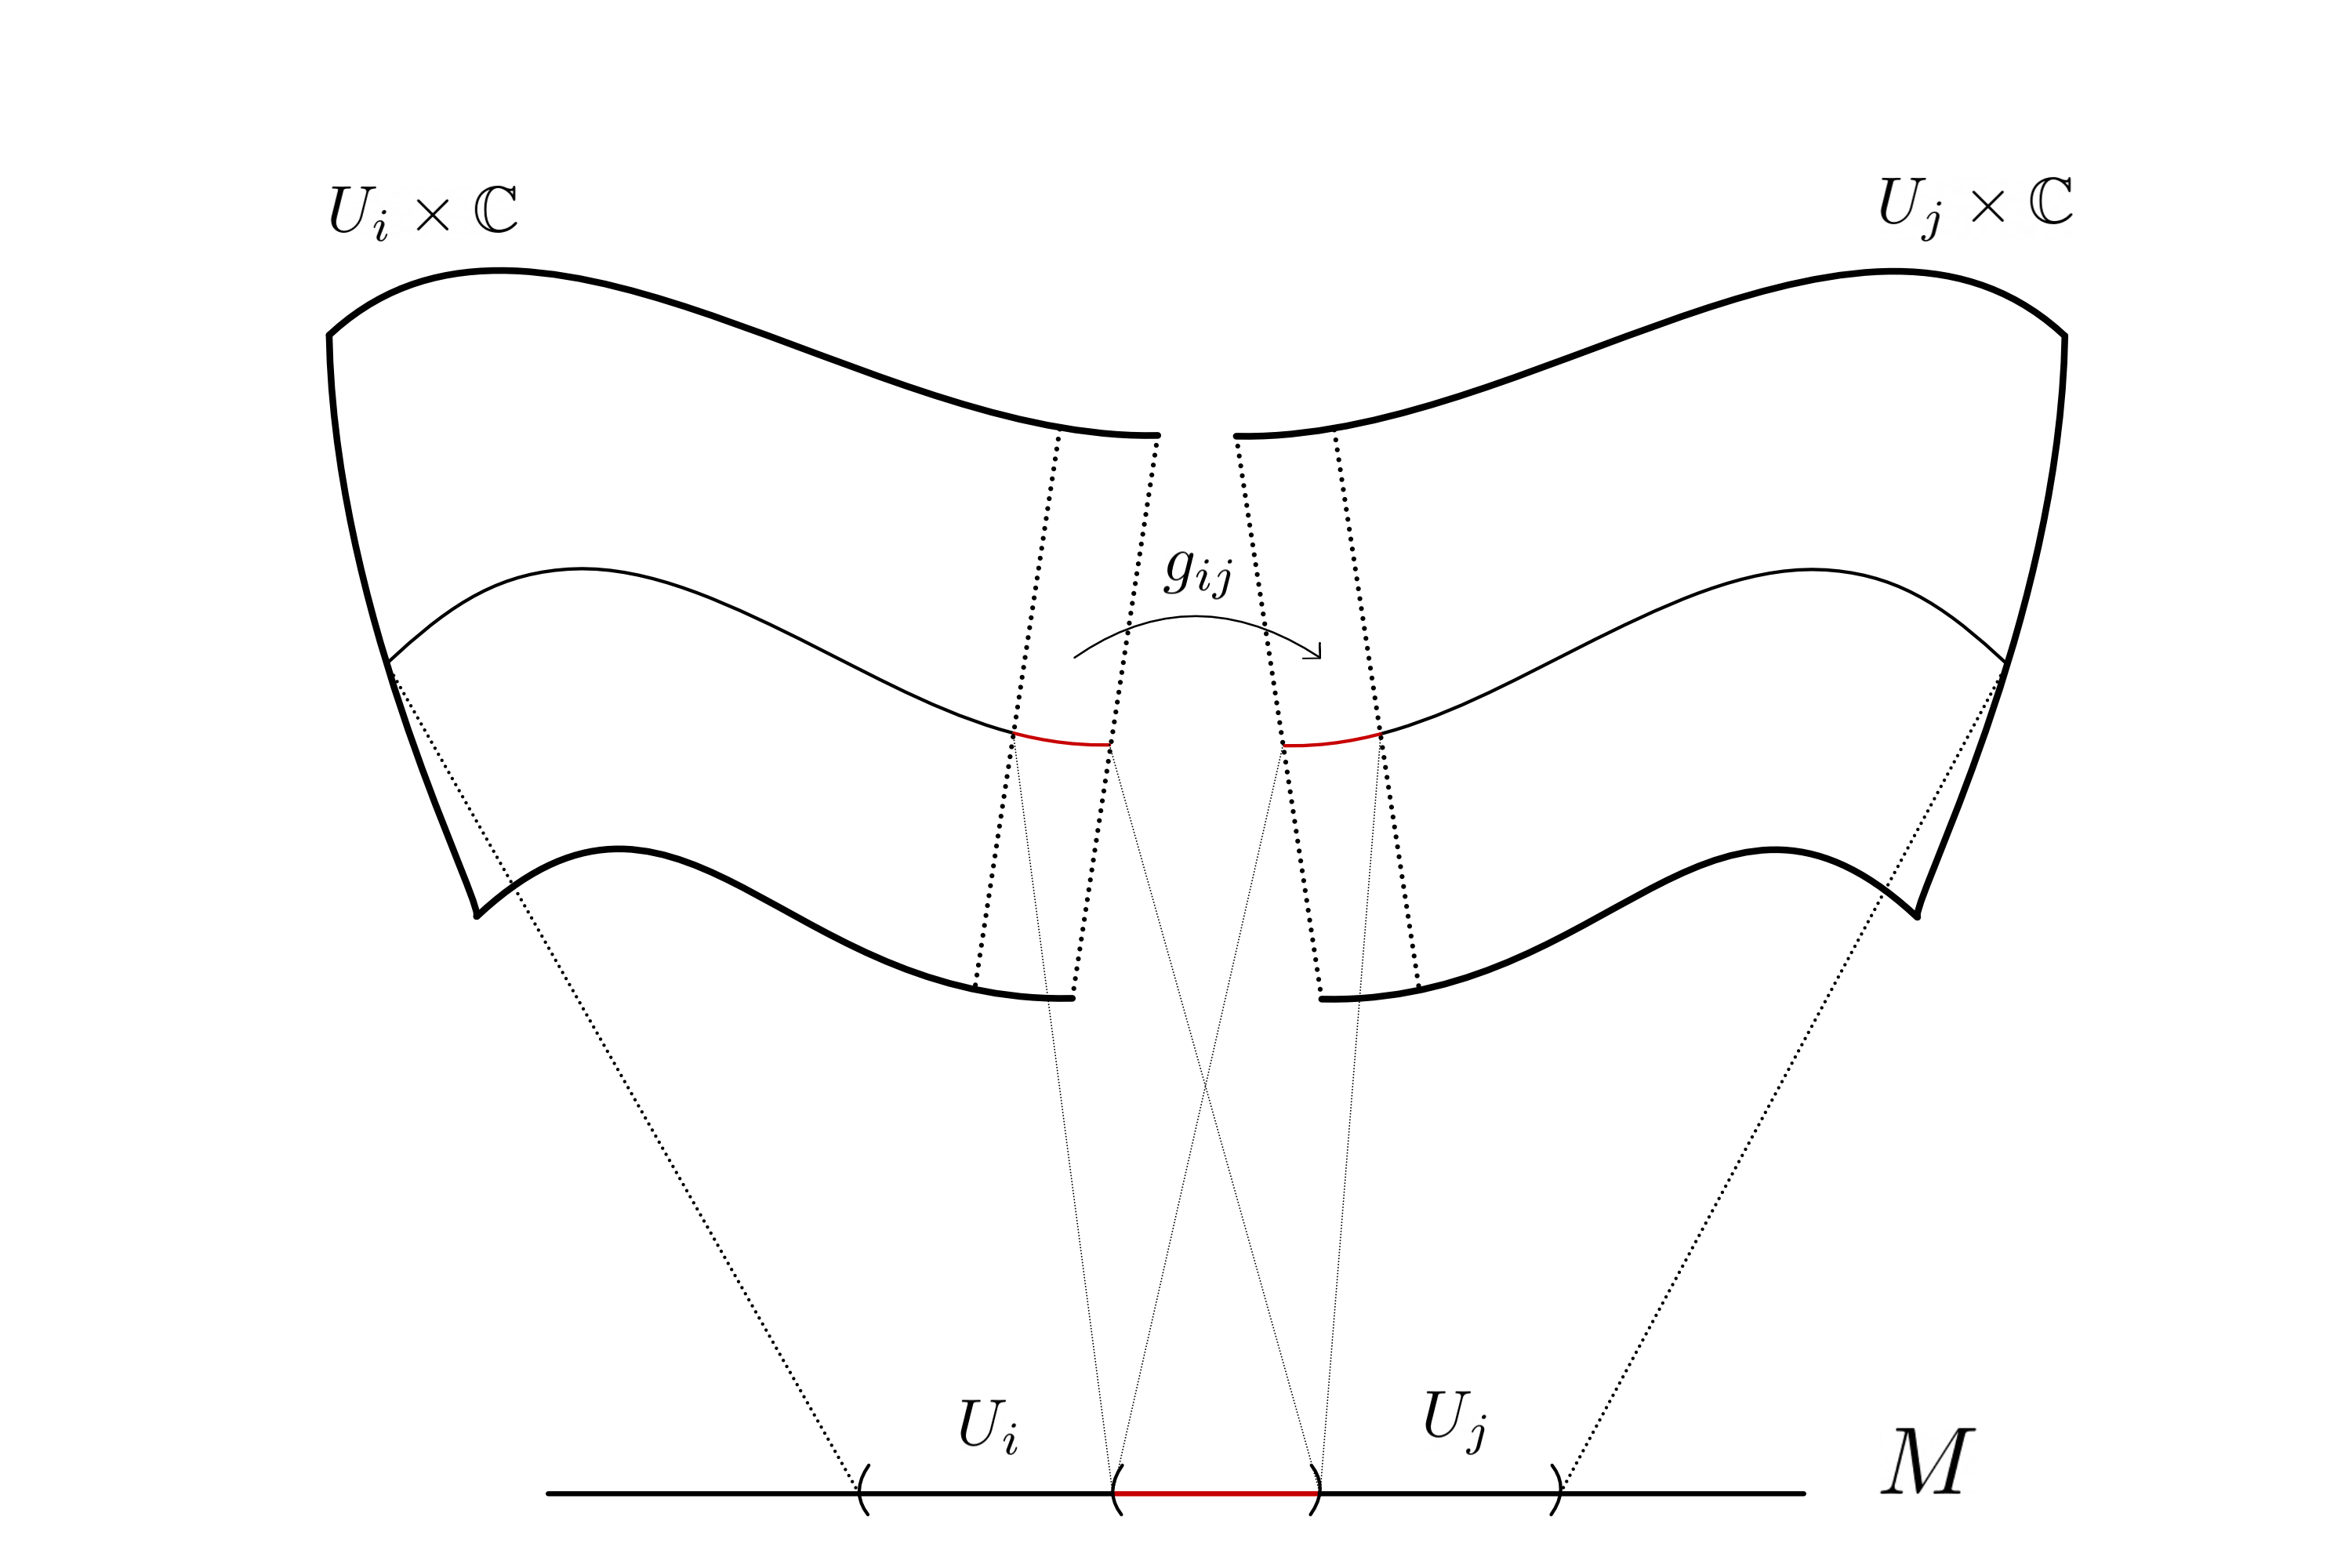
\includegraphics[width=0.5\linewidth]{Imagenes/funciones de transición}
    	\caption{Representación de las funciones de transición}
    	\label{fig:funciones-de-transicion}
    \end{figure}
    
    \begin{remark}\label{cociclos}
    	A las funciones $g_{ij}$ se le llaman \textbf{funciones de transición} y cumplen dos propiedades
    	\begin{align*}
    		g_{ii}&=1,\qquad \text{en }\enspace U_i;\\
    		g_{ij}g_{jk}g_{ki}&=1,\qquad \text{en }\enspace U_i\cap U_j\cap U_k.
    	\end{align*}
    	llamadas \textbf{condiciones de cociclo}.
    \end{remark}

	\begin{example}\label{gijhaztrivial}
		Consideremos el haz trivial $L=M\times \cc$. Por el ejemplo \ref{haztrivial}, sabemos que para cualquier cubierta $\{U_i\}_{i\in I}$ de $M$ se tiene la trivialización
		\begin{align*}
			\psi_i=L|_{U_i}\longrightarrow U_i\times \cc\\
			(p,z)\mapsto (p,z).
		\end{align*}
		Por lo tanto, las funciones de transición de $L$ están dadas por
		\begin{equation*}
			g_{ij}=1,\qquad \text{para todo }i,j\in I.
		\end{equation*}
	\end{example}
	
	Las funciones de transición contienen toda la información necesaria para reconstruir el haz lineal. De hecho, dos haces son isomorfos si y solo si sus funciones de transición representan el mismo cociclo, y recíprocamente, toda colección de funciones que satisfaga las condiciones de cociclo determina un haz lineal.
    
    \begin{propo}[Construcción de un haz holomorfo]
	   Sea $M$ una variedad compleja y $\{U_i\}_{i\in I}$ una cubierta de $M$. Supongamos que para cada $i$ y $j$ tal que $ U_{ij} \neq \emptyset$ tenemos una función holomorfa $g_{ij}:U_{ij}\to \cc^*$ tales que satisfacen las condiciones de cociclos, entonces existe un haz lineal holomorfo $ L\longrightarrow M $ que admite una trivialización en $\{U_i\}_{i\in I}$ y con funciones de transición $g_{ij}$.
    \end{propo}
	\begin{proof}
		\parencite[Chap. 3, Sec. 1, Prop. 3.5]{leecomplex}.
	\end{proof}

\subsection{Operaciones con haces lineales}

	De la proposición anterior se sigue que, para construir un haz lineal, basta definir funciones de transición que satisfagan la condición de cociclo. Esta observación proporciona un método natural para obtener nuevos haces lineales a partir de otros ya dados mediante sus funciones de transición.

\begin{definition}
	Sean $L$ y $L'$ dos haces lineales sobre $M$, con funciones de transición $\{U_i,g_{ij}\}$ y $\{U'_i,g'_{ij}\}$, respectivamente.
	\begin{enumerate}
		\item Definimos el \textbf{haz dual} de $L$, denotado por $L^*$, como el haz lineal cuyas funciones de transición son
		\begin{equation*}
			g_{ij}^{-1}:=\frac{1}{g_{ij}}.
		\end{equation*}
		\item Definimos el \textbf{producto tensorial} $L\otimes L'$ como el haz lineal cuyas funciones de transición son
		\begin{equation*}
			g_{ij}g'_{ij},
		\end{equation*}
		en las intersecciones donde ambas estén definidas\footnote{Las funciones de transición no tienen por qué estar definidas sobre los mismos abiertos. En tal caso, se considera un refinamiento común de las cubiertas, obtenido al intersectar los abiertos de ambas cubiertas.}.
		
		\item Para $k\in \mathbb{N}$, se denota
		\begin{equation*}
			L^{k}:=\underbrace{L\otimes\cdots\otimes L}_{k\text{ veces}},
		\end{equation*}
		al $k$-ésimo producto tensorial de $L$ consigo mismo. Además, usamos la notación 
		\begin{equation*}
			L^{-k}:=(L^*)^k
		\end{equation*}
	\end{enumerate}
\end{definition}	

	
	
	\begin{example}\label{Ltensordual}
		Sea $L$ un haz lineal sobre $M$ con funciones de transición $\{U_i,g_{ij}\}$ de $M$, entonces las funciones de transición de $L\otimes L^*$ están dadas por
		\begin{equation*}
			g_{ij}g_{ij}^{-1}=1,\qquad\text{para todo }i,j\in I.
		\end{equation*}
		Por el ejemplo \ref{gijhaztrivial}, el haz lineal $L\otimes L^*$ corresponde con el haz trivial de $M$.
	\end{example}
	
	\begin{definition}
		Sea $f:N\to M$ una aplicación holomorfa y $\pi:L\to M$ un haz lineal sobre $M$. El \textbf{pullback} de $L$ a través de $f$ es el espacio 
		\begin{equation*}
			f^*L=\{(n,l)\in N\times L: f(n)=\pi(l)\}.
		\end{equation*}
		junto a las aplicaciones naturales
		\begin{align*}
			\pi':f^*L\longrightarrow N\\
			(n,l)\mapsto n
		\end{align*}
		\begin{align*}
			h:f^*L\longrightarrow L\\
			(n,l)\mapsto l
		\end{align*}
		de forma que el siguiente diagrama conmuta
		\begin{center}
			\begin{tikzcd}
				{f ^*L} && L \\
				\\
				N && M
				\arrow["{h}", from=1-1, to=1-3]
				\arrow["{\pi'}"', from=1-1, to=3-1]
				\arrow["\pi", from=1-3, to=3-3]
				\arrow["f"', from=3-1, to=3-3]
			\end{tikzcd}
		\end{center}
	\end{definition}
	
	\begin{remark}
		Si $\{U_i\}_{i\in I}$ es una cubierta de $M$ sobre la cual $L$ se trivializa, con funciones de transición
		\begin{equation*}
				g_{ij}\in \mathcal{O}^*(U_i\cap U_j),
		\end{equation*}
		entonces el pullback $f^*L\to N$ se trivializa sobre la cubierta inducida $\{f^{-1}(U_i)\}_{i\in I}$ de $N$.
		
		En efecto, sobre cada $f^{-1}(U_i)$ definimos la trivialización local de $ f^*L$ usando la trivialización de $L$ sobre $U_i$. Si
		\begin{equation}
			\psi_i:\pi^{-1}(U_i)\longrightarrow U_i\times \mathbb{C}
		\end{equation}
		es una trivialización de $L$, entonces se obtiene una trivialización de $f^*L $ sobre $f^{-1}(U_i) $ dada por
		\begin{align*}
			\widetilde{\psi}_i:f^*L|_{f^{-1}(U_i)}&\longrightarrow f^{-1}(U_i)\times \mathbb{C}\\
			(n,\ell)&\mapsto \bigl(n, z\bigr),
		\end{align*}
		donde $\psi_i(\ell)=(f(n),z)$. Ahora, en una intersección $f^{-1}(U_{ij})$, el cambio de trivialización viene dado por
		\begin{equation*}
			\widetilde{\psi}_i\circ \widetilde{\psi}_j^{-1}(n,z)=\bigl(n, (g_{ij}\circ f)(n) z\bigr).
		\end{equation*}
		Por tanto, las funciones de transición del pullback $f^*L$ son precisamente
		\begin{equation*}
			(f^*g)_{ij}=g_{ij}\circ f
			\quad\text{en}\quad
			f^{-1}(U_{ij}).
		\end{equation*}
	\end{remark}

\subsection{Espacio de secciones}

	\begin{definition}
		Sea $\pi:L\to M$ un haz lineal sobre una variedad compleja $M$. Una \textbf{sección} (global) de $L$ es una aplicación holomorfa $s:M\to L$ tal que
		\begin{equation*}
			\pi\circ s=\mathrm{id}_M.
		\end{equation*}
		Una \textbf{sección local} es una sección $s:U\to L$ definida solo en un abierto $U\subset M$. 
		\begin{figure}[H]
			\centering
			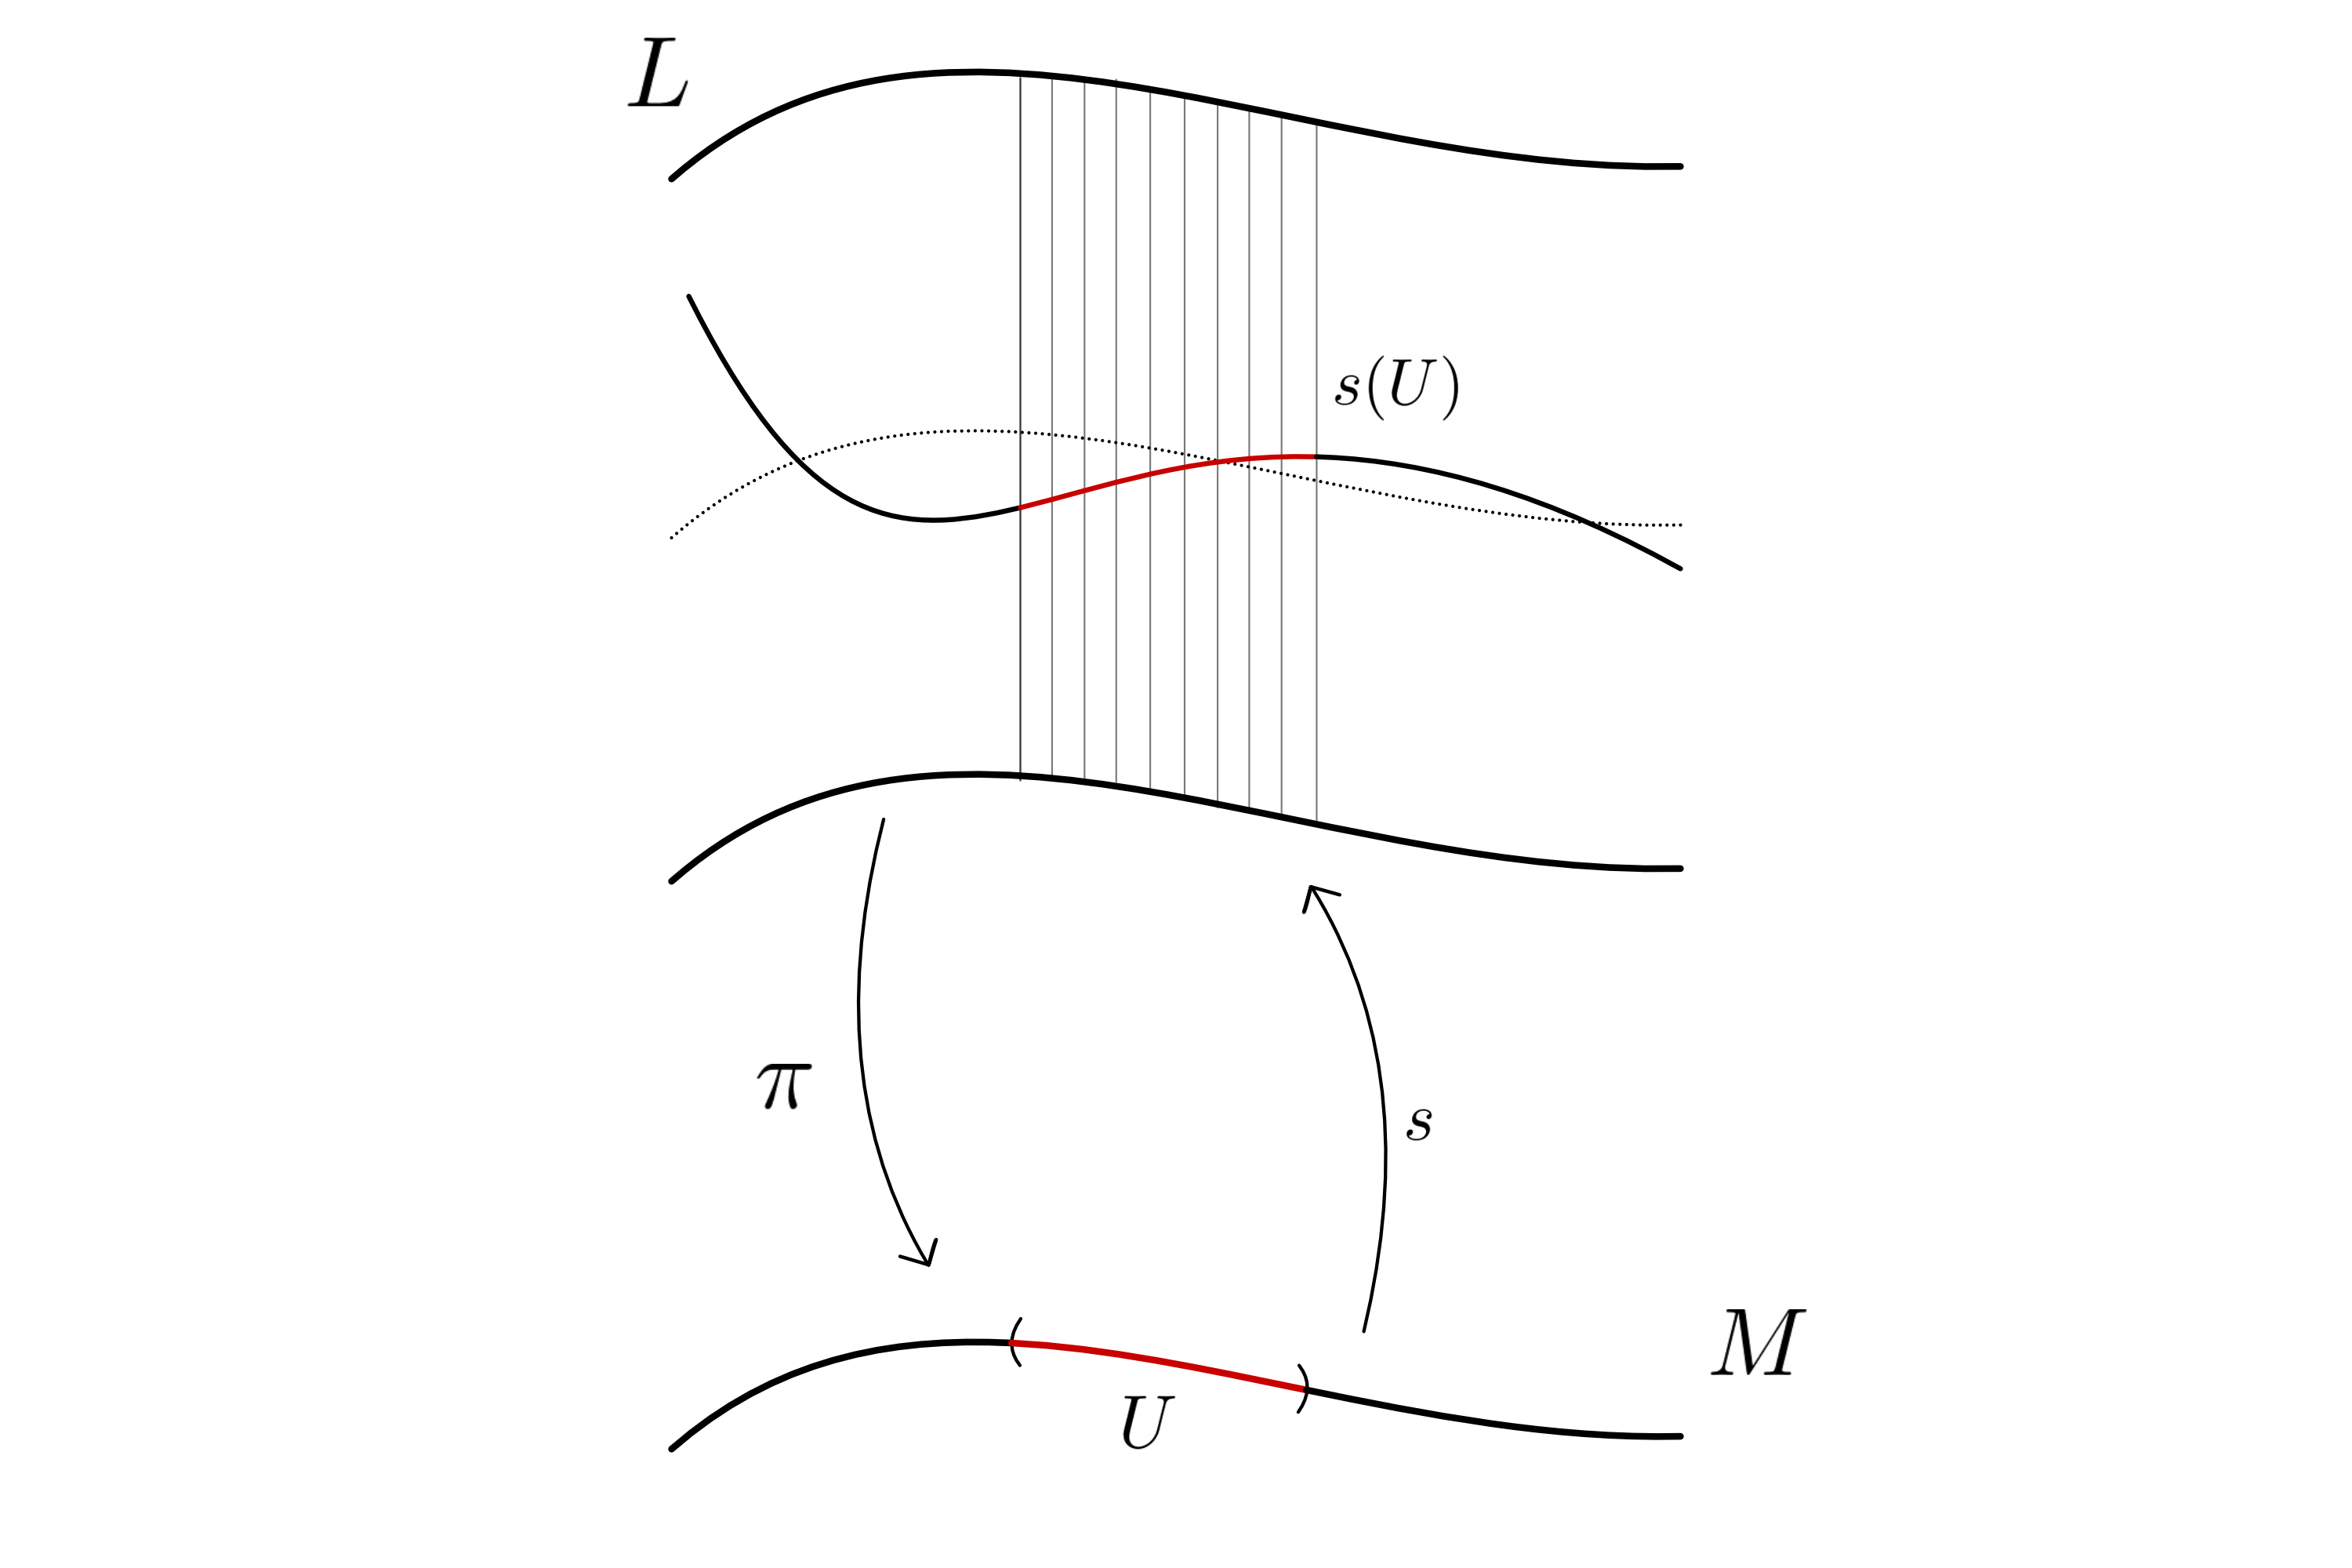
\includegraphics[width=0.5\linewidth]{Imagenes/seccion local}
			\caption{Interpretación de las secciones locales}
			\label{fig:seccion-local}
		\end{figure}
		
	\end{definition}
	
	Si $p\in M$ y $s:M\to L$ es una sección global, entonces $\pi(s(p))=p$. Así, $s(p)\in \pi^{-1}(p)=L_p$. Esto significa que las secciones $s$ siempre mandan a los puntos $p\in M$ a sus fibras $L_p$. Entonces, podemos pensar que una sección encaja a $M$ dentro de $L$ de manera que intersecta solo una vez a cada fibra. En particular, existe siempre una sección $s_0:M\to L$ definida como
	\begin{equation*}
		s_0(p)=0\in L_p,\qquad \text{para todo }p\in M.
	\end{equation*}
	La sección $s_0$ es llamada \textbf{sección cero} de $L$.
	
	\begin{definition}
		Sea $M$ una variedad compleja y $\pi:L\to M$ un haz lineal. Definimos el \textbf{espacio de secciones holomorfas} como
		\begin{equation*}
			\oo(U;L):=\{s:U\to L: s\text{ es una sección local de }L\}.
		\end{equation*}
	\end{definition}
	
	\begin{remark}\label{seccionlocalholomorfa}
		Sea $\pi:L\to M$ un haz lineal y $s:U\to L$ una sección local. Por definición
		\begin{equation}\label{pis(p)}
			\pi \circ s(p)=p,\qquad p\in U.
		\end{equation} 
		Supongamos que $L$ se trivializa en $U$, entonces
		\begin{equation*}
			\psi:\pi^{-1}(U)\cong U\times \cc.
		\end{equation*}
		Como $s(p)$ pertenece a la fibra de $p$, tenemos que
		\begin{equation*}
			s(p)\in \pi^{-1}(U)\cong U\times \cc.
		\end{equation*}
		Por (\ref{pis(p)}), tenemos que $s$ conmuta con la proyección a la primera entrada. Por lo que
		\begin{equation*}
			\psi(s(p))=(p,z)\in U\times \cc.
		\end{equation*}
		Como $s$ es holomorfa, existe una función holomorfa $f\in \oo_M(U)$ tal que
		\begin{equation*}
			\psi(s(p))=(p,f(p)).
		\end{equation*}
		Más aún, consideremos una intersección de abiertos trivializantes $U_i\cap U_j$ con funciones de transición $g_{ij}$. Entonces
		\begin{equation*}
			\psi_i(s(p))=(p,f_i(p)),\qquad \psi_j(s(p))=(p,f_j(p)).
		\end{equation*}
		Por definición de las funciones de transición
		\begin{equation*}
			\psi_i\circ \psi_j^{-1}(p,z)=(p,g_{ij}(p)z).
		\end{equation*}
		De esta manera,
		\begin{equation*}
			(p,f_i(p))=\psi_i(s(p))=\psi_i(\psi_j^{-1}(p,f_j(p)))=(p,g_{ij}(p)f_j(p)).
		\end{equation*}
		Por lo tanto, 
		\begin{equation*}
			f_i(p)=g_{ij}(p)f_j(p).
		\end{equation*}
	\end{remark}
	
	Notemos que las secciones holomorfas de un haz lineal pueden sumarse y multiplicarse por escalares complejos, gracias a la estructura de $\cc$-espacio vectorial de las fibras. Además, por la observación anterior, estas operaciones preservan la holomorfía, pues se reducen punto a punto a operaciones entre funciones holomorfas. En consecuencia, tenemos lo siguiente:
	
	\begin{propo}
		Sea $M$ una variedad compleja y $\pi:L\to M$ un haz lineal. Entonces el funtor definido por
		\begin{align*}
			\mathcal{O}(L)(U):=\mathcal{O}(U;L)
		\end{align*}
		para todo abierto $U$ de $M$, es una gavilla de $\cc$-espacios vectoriales.
	\end{propo}
	
	La demostración de esta proposición es análoga a la de la gavilla de funciones holomorfas. Además, las secciones holomorfas pueden multiplicarse por funciones holomorfas locales y el resultado sigue siendo una sección holomorfa. Esto muestra que la gavilla $\mathcal{O}(L)(\_)$ posee de manera natural una estructura de gavilla de $\mathcal{O}_M$-módulos. En particular, por la observación \ref{seccionlocalholomorfa}, dicha gavilla es localmente isomorfa a $\mathcal{O}_M$; es decir, $\mathcal{O}(L)(\_)$ es una gavilla de $\mathcal{O}_M$-módulos localmente libre de rango $1$. Por lo tanto, $\mathcal{O}(L)(\_)$ es una gavilla coherente (véase \parencite[Chap.~5, Sec.~3.4]{griffiths}).

	\begin{example}\label{seccionesdeltrivial}
		Consideremos el haz trivial $L$ sobre $M$ y tomemos $U$ un abierto no vacío de $M$. Entonces
		\begin{equation*}
			\pi^{-1}(U)= U\times \cc.
		\end{equation*}
		Por la observación \ref{seccionlocalholomorfa}, tenemos que si $s$ es una sección local sobre $U$ entonces
		\begin{equation*}
			s(p)=(p,f(p)),\qquad \text{para todo }\ p\in U,
		\end{equation*}
		donde $f\in\oo_M(U)$. De esta manera, $s$ está totalmente determinada por la función holomorfa $f$. Asimismo, toda función holomorfa $f$ de $M$ determina una sección local de $L$. Por lo tanto, la gavilla $\mathcal{O}(L)$ corresponde con la gavilla de funciones holomorfas $\oo_M$.
	\end{example}
	
	\begin{theorem}
		Sea $M$ una variedad compleja compacta y $\pi:L\to M$ un haz lineal. Entonces el espacio de secciones globales $	H^0(M,L):=\mathcal{O}(M;L)$ \footnote{La notación proviene del hecho de que el espacio de secciones globales coincide con el grupo de cohomología de Čech de grado $0$ de la gavilla asociada al haz lineal $L$.} es un $\cc$-espacio vectorial de dimensión finita.
	\end{theorem}
	
	Este resultado muestra nuevamente la rigidez de la geometría compleja, pues aunque un haz lineal pueda admitir muchas secciones locales, la compacidad de la variedad impone una fuerte restricción sobre las secciones holomorfas globales. En general, la finitud de $H^0(M,L)$ se deduce del hecho de que la gavilla $\mathcal{O}(L)(\_)$ es coherente (véase \parencite[Chap.~VIII, Sec.~A, Cor.~10]{gunningrossi}). Sin embargo, también puede obtenerse mediante argumentos analíticos más elementales, introduciendo una norma global sobre $\mathcal{O}(M;L)$ y demostrando que la bola unitaria cerrada es compacta (véase \parencite[Chap.~3, Sec.~1, Theo.~3.13]{leecomplex}).
	
	\begin{example}\label{H0deltrivial}
		Consideremos el haz trivial $L$ sobre $M$. Por el ejemplo \ref{seccionesdeltrivial} tenemos que
		\begin{equation*}
			H^0(M,L)\cong \oo_M(M).
		\end{equation*} 
		Si $M$ es compacta, toda función holomorfa global es constante (véase teorema \ref{holomorfasglobal}), luego
		\begin{equation*}
			H^0(M,L)\cong\cc.
		\end{equation*}
		Por lo tanto,
		\begin{equation*}
			\dim_\cc H^0(M,L)=1.
		\end{equation*}
	\end{example}
	
	\begin{example}[Secciones del pullback]\label{seccionespullback}
		Sea $f:N\to M$ una aplicación holomorfa y $\pi:L\to M$ un haz lineal. Recordemos que el pullback está dado por
		\begin{equation*}
			f^*L=\{(n,l)\in N\times L:f(n)=\pi(l)\}.
		\end{equation*}
		Sea $s\in H^0(M,L)$ una sección global de $L$. Definamos
		\begin{align*}
			f^*s&:N\longrightarrow f^*L\\
			f^*s(n)&=(n,s(f(n))).
		\end{align*}	
		Es inmediato que $f^*s$ es holomorfa y 
		\begin{equation*}
			(\pi'\circ f^*s)(n)=\pi'(f^*s(n))=\pi'(n,s(f(n)))=n.
		\end{equation*}
		De esta manera, $f^*s$ es una sección global de $f^*L$. Notemos además que esta construcción determina una aplicación $\cc$-lineal
		\begin{equation*}
			f^*:H^0(M,L)\longrightarrow H^0(N,f^*L).
		\end{equation*}
		En general, $f^*$ no es sobreyectiva. Por ejemplo, tomemos $M=\{\mathrm{pt}\}$ y $L=\cc$ es haz trivial sobre $M$. Entonces $H^0(M,L)\cong\cc$, mientras que para cualquier variedad compleja $N$ se tiene que
		\begin{equation*}
			H^0(N,f^*L)\cong H^0(N,N\times \cc)=\oo_N(N).
		\end{equation*} 
		Tomando $N=\cc$, entonces $\oo_N(N)$ tiene dimensión infinita pues $N$ no es compacta. Por lo que $f^*$ determina un morfismo lineal
		\begin{equation*}
			\cc\longrightarrow \oo(\cc).
		\end{equation*}
		el cual no es sobreyectivo.
	\end{example}
	
\section{Haces amplios y encajes}

Los haces lineales son importantes en el estudio de los encajes al espacio proyectivo porque actúan como el mecanismo que nos permite construir aplicaciones holomorfas desde una variedad compleja hacia $\pp^N$. Sin la estructura de los haces lineales, no existiría una forma natural de generar las coordenadas homogéneas necesarias para \enquote{sumergir} una variedad compleja en el mundo algebraico del espacio proyectivo. 

\subsection{Haces lineales del espacio proyectivo}

	Consideremos el espacio proyectivo $\pp^n$ y definamos el conjunto
	\begin{equation*}
		\mathcal{O}(-1)=\{(l,z)\in\pp^n\times \cc^{n+1}:l\in\pp^n, z\in l\text{ ó }z=0\}.
	\end{equation*}
	Notemos que la proyección a la primera entrada $\pi:\mathcal{O}(-1)\to\pp^n$ es una aplicación holomorfa sobreyectiva. Con esto podemos ver que:
	
	\begin{propo}
		$\mathcal{O}(-1)$ es un haz lineal del espacio proyectivo $\pp^n$.
	\end{propo}
	\begin{proof}
		Sea $l\in\pp^n$, entonces la fibra $\pi^{-1}(l)$ es el conjunto de puntos $z\in\cc^{n+1}$ que pertencen a la línea compleja $l$. Con lo cual,
		\begin{equation*}
			\pi^{-1}(l)\cong \cc.
		\end{equation*}
		Consideremos $\pp^n=\bigcup_{i=0}^n U_i$ la cubierta estandar afin del espacio proyectivo. 
%		Una trivialización canónica de $\oo(-1)$ sobre la cubierta es
%		\begin{align*}
%			\psi_i:\pi^{-1}(U_i)\longrightarrow U_i\times\cc\\
%			(l,z)\mapsto (l,\mathrm{pr}_i(z))
%		\end{align*}
%		donde $z=(z_0,\dots,z_n)$. 
		
		Determinemos sus funciones de transición a partir de trivializaciones locales. Para cada abierto $U_i$, definimos
		\begin{equation*}
			\psi_i:\pi^{-1}(U_i)\longrightarrow U_i\times \cc
		\end{equation*}
		mediante
		\begin{equation*}
			\psi_i(l,w)=
			\left(
			l,
			\frac{w_i}{z_i}
			\right),
		\end{equation*}
		donde $w=(w_0,\dots,w_n)\in l$. Esta expresión está bien definida, pues como $w$ pertenece a la recta $l$, existe $\lambda\in\cc$ tal que $w=\lambda z$, y por tanto
		\begin{equation*}
			\frac{w_i}{z_i}=\lambda.
		\end{equation*}
		La inversa de $\psi_i$ está dada por
		\begin{equation*}
			\psi_i^{-1}([z],\lambda)=([z],\lambda z),
		\end{equation*}
		de modo que $\psi_i$ es una trivialización holomorfa.
		
		Ahora, sobre la intersección $U_i\cap U_j$, el cambio de trivialización
		\begin{equation*}
			\psi_i\circ \psi_j^{-1}:
			(U_i\cap U_j)\times\cc
			\longrightarrow
			(U_i\cap U_j)\times\cc,
		\end{equation*}
		está dado por
		\begin{equation*}
			\psi_i\circ \psi_j^{-1}([z],\lambda)
			=\left([z],\frac{z_j}{z_i}\lambda \right).
		\end{equation*}
		Por lo tanto, las funciones de transición de $\mathcal{O}(-1)$ son
		\begin{equation*}
			g_{ij}=\frac{z_j}{z_i}.
		\end{equation*}
	\end{proof}
	
	\begin{figure}
		\centering
		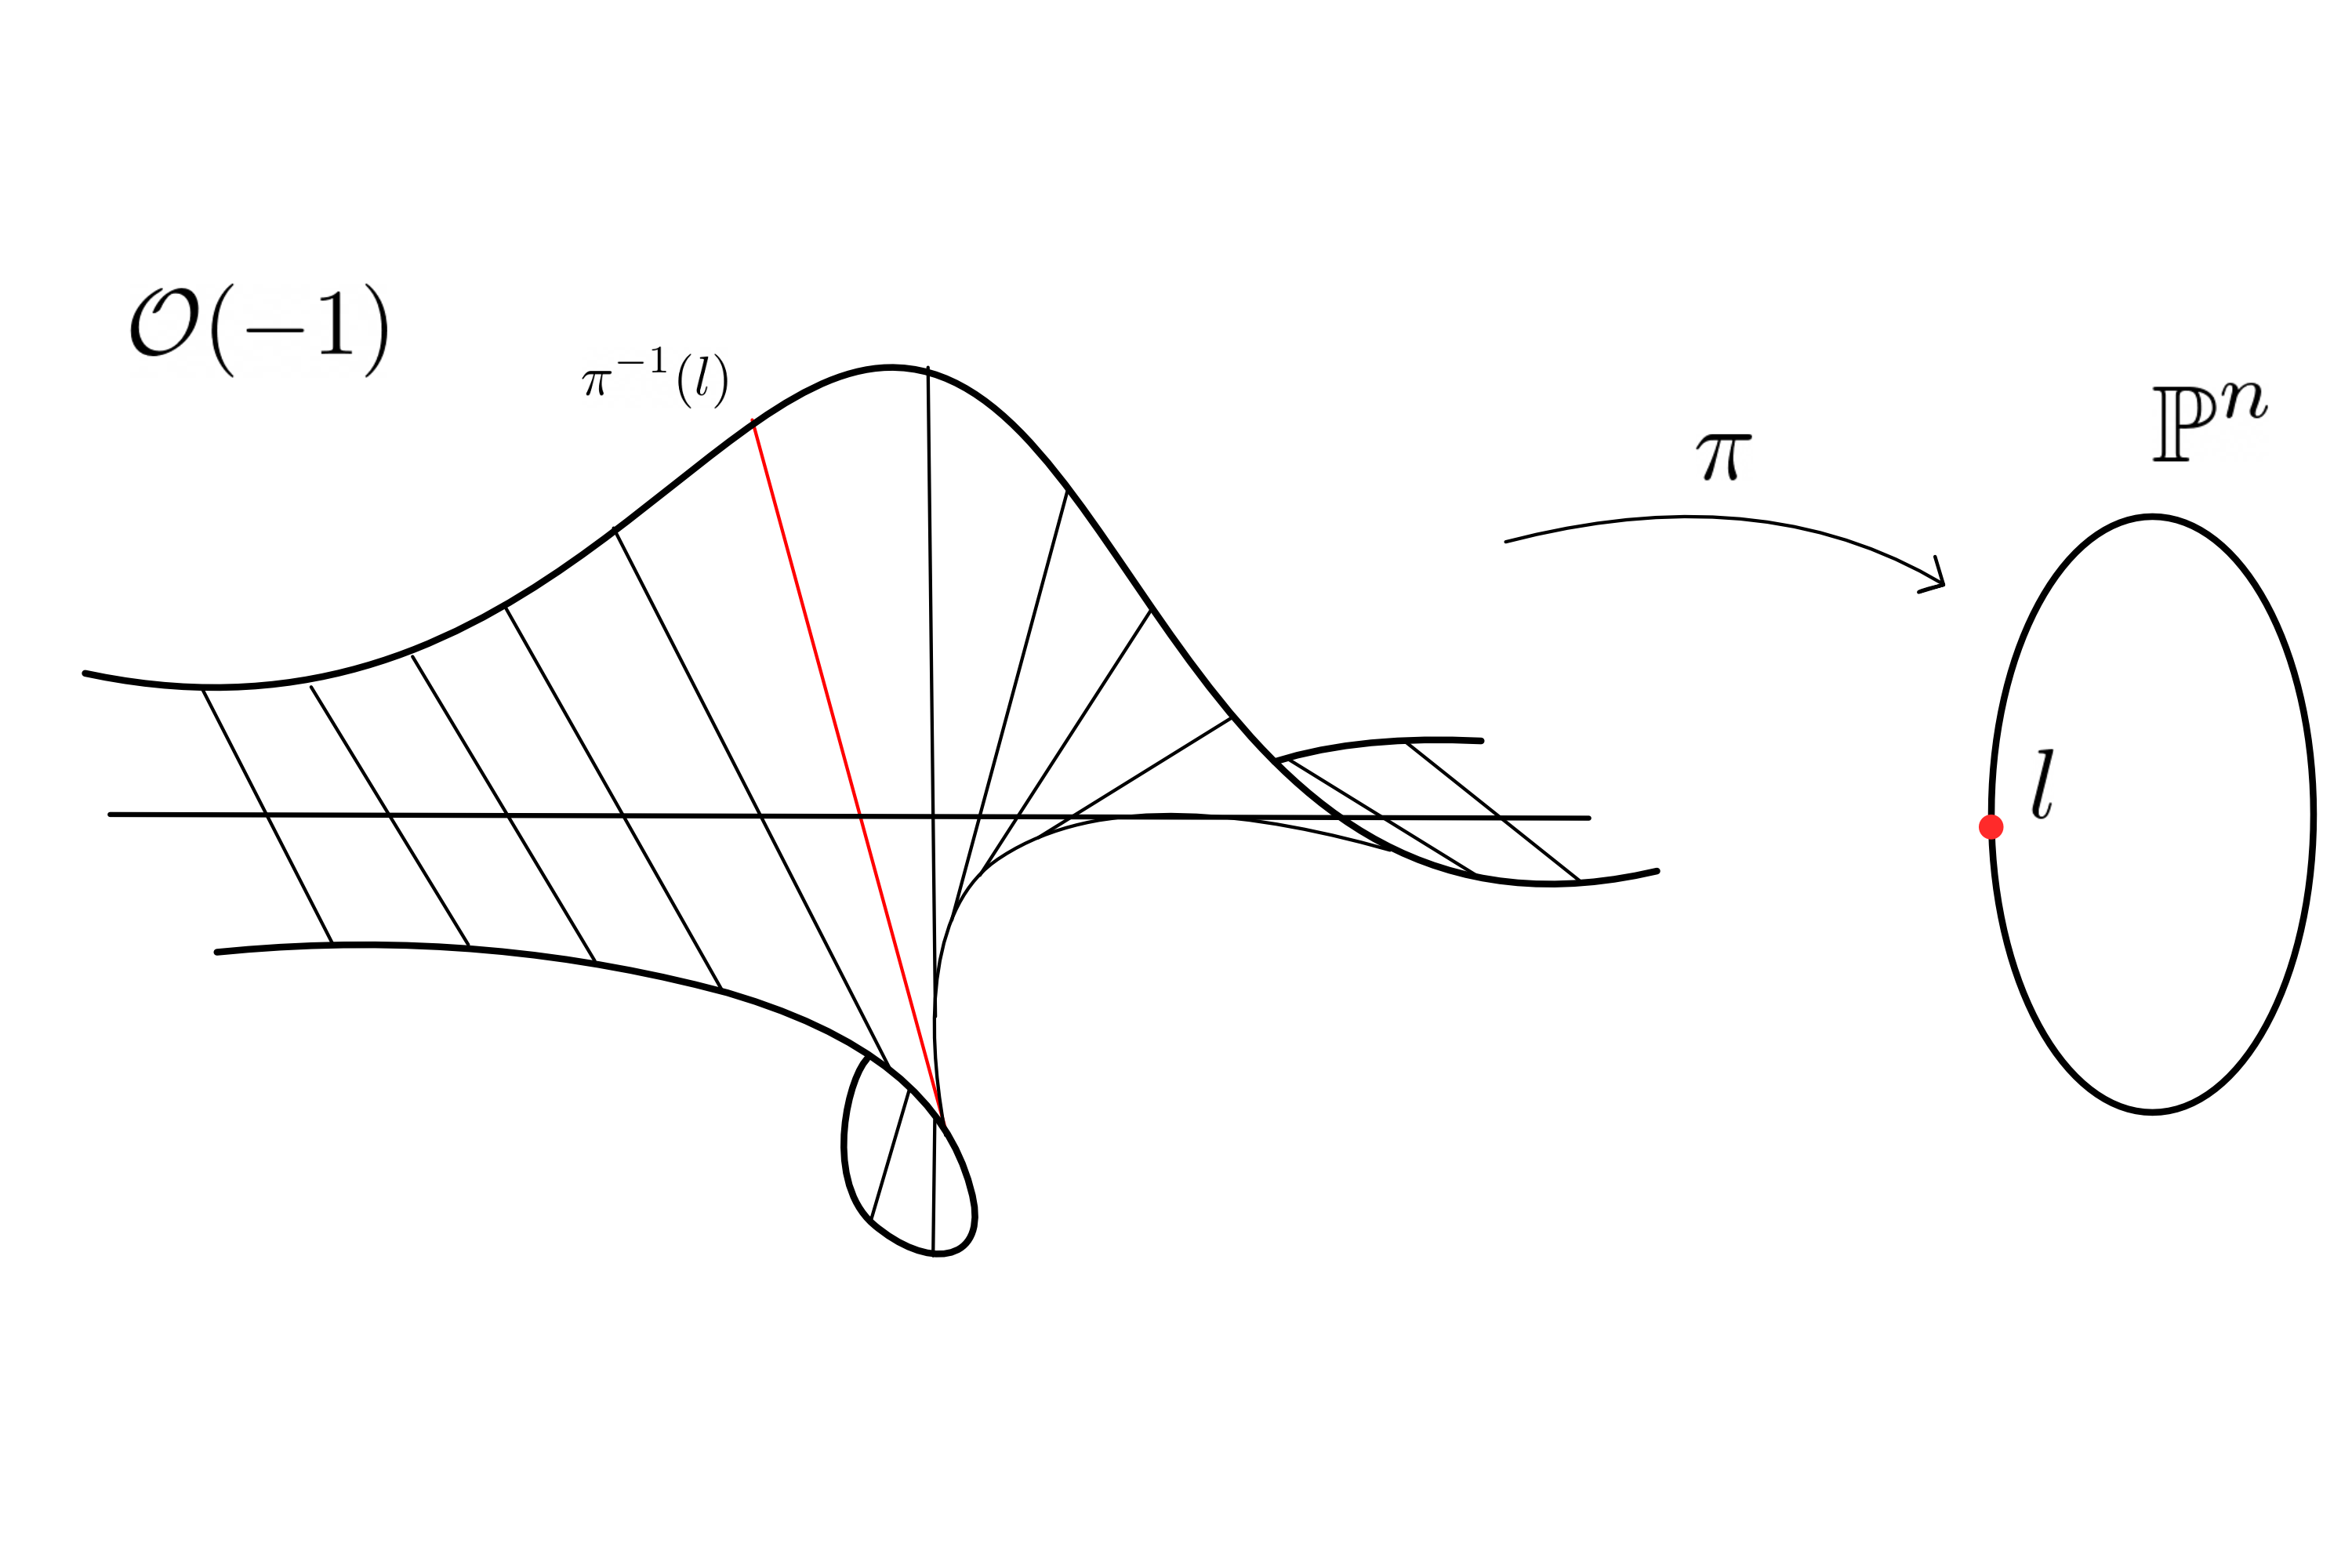
\includegraphics[width=0.7\linewidth]{Imagenes/tautologico}
		\caption{Interpretación geométrica del haz lineal $\mathcal{O}(-1)$.}
		\label{fig:tautologico}
	\end{figure}
	
	
	\begin{definition}
		Consideremos el haz lineal $\oo(-1)$ sobre el espacio proyectivo $\pp^n$.
		\begin{enumerate}
			\item El haz lineal $\mathcal{O}(-1)$ es llamado \textbf{haz tautológico}.
			\item El haz dual $\mathcal{O}(1):=\mathcal{O}(-1)^*$ es llamado \textbf{haz de hiperplanos}.
			\item El haz trivial sobre $\pp^n$ lo denotamos como $\mathcal{O}(0):=\pp^n\times\cc$.
			\item La potencia tensorial la denotamos como $\mathcal{O}(-d):=\mathcal{O}(-1)^d$ y  $\mathcal{O}(d):=\mathcal{O}(1)^{d}$.
		\end{enumerate}
	\end{definition}

	\begin{lemma}\label{seccionesnotriviales}
		Sea $L$ un haz lineal holomorfo sobre una variedad compleja conexa compacta $M$. Entonces $L$ es trivial si, y solo si, $L$ y su dual $L^*$ admite secciones globales no triviales.  
	\end{lemma}
	\begin{proof}
		Supongamos que $L$ es trivial. Por el ejemplo \ref{seccionesdeltrivial}, $L$ admite secciones constantes no cero. Además, el dual $L^*$ vuelve a ser $L$, por lo que $L^*$ también admite secciones constantes no cero.
		
		Ahora supongamos que $L$ y $L^*$ admite secciones globales no cero. Tomemos las secciones globales no cero
		\begin{equation*}
			s\in H^0(M,L),
			\qquad
			t\in H^0(M,L^*).
		\end{equation*}
		Entonces por el ejemplo \ref{Ltensordual} tenemos que
		\begin{equation*}
			s\otimes t\in H^0(M,L\otimes L^*)\cong H^0(M,\oo_M).
		\end{equation*}
		Eso significa que $s\otimes t$ corresponde con una función holomorfa global $f\in \oo_M(M)$. Por el teorema \ref{holomorfasglobal}, $s\otimes t$ es constante. 
		
		Como $s$ y $t$ son holomorfas no cero, siempre existe $r\in M$ tal que $s(r)\neq 0$ y $t(r)\neq o$. Con lo cual $(s\otimes t)(r)\neq 0$. De esta manera, $s\otimes t\neq 0$. En particular, $s(p)\neq 0$ para todo punto $p\in M$.
		
		Ahora bien, una sección global que nunca se anula trivializa globalmente al haz $L$. Definamos
		\begin{align*}
			\Psi:M\times \cc\longrightarrow L,\\
			\Psi(p,\lambda)=\lambda s(p).
		\end{align*}
		Consideremos una trivialización local $(U,\psi)$ de $L$, entonces
		\begin{equation*}
			s|_U(p)=(p,f(p)),\qquad \text{para todo }\ p\in U
		\end{equation*}
		donde $f\in\oo_M(U)$. Como $s$ nunca se anula, entonces $f$ tampoco nunca se anula. Además, como $L|_U=\pi^{-1}(U)\cong U\times \cc$, entonces a todo punto $x\in L|_U$ se le asocia de manera única un punto $(q,\lambda')\in U\times \cc$. De esta manera, podemos definir $\Psi^{-1}$ localmente como
		\begin{equation*}
			\Psi|_U^{-1}(x)=\left(q,\frac{\lambda'}{f(q)}\right),
		\end{equation*}
		la cual está bien definida porque $f$ nunca se anula.
		Notemos que en efecto es la inversa, pues
		\begin{align*}
			\Psi\circ\Psi^{-1}(x)=\Psi\left(q,\frac{\lambda'}{f(q)}\right)=\frac{\lambda'}{f(q)}s(q)=\frac{\lambda'}{f(q)}(q,f(q))=\left(q,\frac{\lambda'}{f(q)}f(q)\right)=(q,\lambda')=x,\\
			\Psi^{-1}\circ\Psi(p,\lambda)=\Psi^{-1}(\lambda s(p))=\Psi^{-1}(\lambda(p,f(p)))=\Psi^{-1}(p,\lambda f(p))=\left(p,\frac{\lambda f(p)}{f(p)}\right)=(p,\lambda).
		\end{align*}
		Por lo tanto, $\Psi:M\times \cc\to L$ es un biholomorfismo y $L$ es trivial.
	\end{proof}
	
	Con este lema, podemos probar uno de los resultados más importante de los haces lineales del espacio proyectivo.
	
	\begin{theorem}\label{seccionesproyectivo}
		Consideremos el haz lineal $\oo(1)$ del espacio proyectivo $\pp^n$ y sea $d$ un entero positivo no cero. Entonces se cumple lo siguiente:
		\begin{enumerate}
			\item $H^0(\pp^n, \mathcal{O}(d))\cong \cc[z_0,\cdots,z_n]_{(d)}$
			\item $H^0(\pp^n, \mathcal{O}(0))\cong \cc$
			\item $H^0(\pp^n, \mathcal{O}(-d))\cong\{0\}$
		\end{enumerate}
	\end{theorem}
	\begin{proof} $ $
		\begin{enumerate}
			\item Recordemos que el conjunto $\cc[z_0,\cdots,z_n]_{(d)}$ es el anillo de polinomios homogéneos de grado $d$.
			
			Consideremos la cubierta estandar afín de $\pp^n$
			\begin{equation*}
				\pp^n=\bigcup_{i=0}^n U_i.
			\end{equation*}
			En una intersección $U_j\cap U_k$, las funciones de transición de $\mathcal{O}(-1)$ están dadas por 
			\begin{equation*}
				g_{ij}=\frac{z_j}{z_i}.
			\end{equation*}
			Entonces las funciones de transición de $\mathcal{O}(d)$ son de la forma
			\begin{equation*}
				g'_{ij}=\frac{z_k^d}{z_j^d}.
			\end{equation*}
			Por la observación \ref{seccionlocalholomorfa}, toda sección global $s\in H^0(M,L)$ está determinada por una colección de funciones holomorfas $f_i\in\oo_{\pp^n}(U_i)$ tal que $f_j=\frac{z_k^d}{z_j^d}f_k$ en $U_i\cap U_j$. Consideremos la aplicación cociente
			\begin{align*}
				q:\cc^{n+1}\setminus\{0\}\longrightarrow \pp^n,
			\end{align*}
			entonces el pullback $f'_j=f_j\circ q$ está bien definida y holomorfa cuando $z_j\neq 0$. De la relación
			\begin{equation*}
				z_j^df'_j=z_k^d f'_k
			\end{equation*}
			tenemos que la función
			\begin{equation*}
				F(z):=z_j^df_j([z])
			\end{equation*}
			no depende del índice $j$. Así, $F$ es holomorfa en $\cc^{n+1}\setminus\{0\}$. Por el teorema de Hartog \ref{hartogs}, esta función se extiende holomorfamente a $\cc^{n+1}$. Además, satisface la condición de homogeneidad 
			\begin{equation*}
				F(\lambda z)=(\lambda z_j)^d f_j([\lambda z])=\lambda^d F(z),\qquad \lambda\in\cc^*.
			\end{equation*}
			Al expandir en serie de potencias, esta identidad fuerza que solo aparezcan monomios de grado $d$. 
			Escribiendo
			\begin{equation*}
				F=\sum_\alpha a_\alpha z^\alpha,
			\end{equation*}
			la identidad $ F(\lambda z)=\lambda^dF(z)$ implica que
			\begin{equation*}
				\sum_\alpha a_\alpha \lambda^{|\alpha|}z^\alpha
				=
				\sum_\alpha a_\alpha \lambda^d z^\alpha.
			\end{equation*}
			Por unicidad de la serie de potencias,
			$a_\alpha=0$ si $|\alpha|\neq d$. Con lo cual, $F$ es un polinomio homogéneo de grado $d$.
			
			Consideremos un polinomio $P$ homogéneo de grado $d$, entonces en cada abierto $U_j$ podemos definir
			\begin{equation*}
				f_j([z])=\frac{P(z)}{z_j^d}.
			\end{equation*}
			Esta función es holomofa en $U_j$, y la expresión coincide en las intersecciones pues $P$ es un polinomio homogéneo de grado $d$. Por lo tanto, la colección $\{f_j\}_{j=0}^n$ determina una sección global holomorfa de $\mathcal{O}(d)$.
			
			\item Se sigue del ejemplo \ref{H0deltrivial}.
			
			\item Se sigue del lema \ref{seccionesnotriviales}.
		\end{enumerate}
	\end{proof}
	
\subsection{Aplicación asociada a un haz}


    \begin{definition}[Puntos base]
		Sea $L$ un haz lineal sobre una variedad compleja conexa $M$. El conjunto de \textbf{puntos bases} de $L$ está dado por
		\begin{equation*}
			\mathrm{Bs}(L)=\{p\in M:s(p)=0\text{ para todo }s\in H^0(M,L)\},
		\end{equation*}
		donde $s(p)=0$ signifa que la sección $s$ coincide con la sección cero $s_0\in H^0(L,M)$ en el punto $p$.
	\end{definition}

	\begin{remark}
		Sea $L$ un haz lineal sobre una variedad compleja conexa $M$. Para cada sección global $ s\in H^0(M,L) $, su conjunto de ceros
		\begin{equation*}
			Z(s)=\{p\in M: s(p)=0\}
		\end{equation*}
		es un subconjunto cerrado de $M$. En efecto, localmente $L$ se trivializa, y bajo una trivialización $s$ se identifica con una función 
		holomorfa. Por definición,
		\begin{equation*}
			\mathrm{Bs}(L)=\bigcap_{s\in H^0(M,L)} Z(s).
		\end{equation*}
		La intersección arbitraria de cerrados es cerrada, entonces $\mathrm{Bs}(L)\subset M$ es un subconjunto cerrado.\\
		De esta manera, el abierto
		\begin{equation*}
			U:=M\setminus \mathrm{Bs}(L).
		\end{equation*}
		es una variedad compleja por ser un abierto de una variedad compleja.
%		Por definición de $ \mathrm{Bs}(L) $, para todo $ p\in U $ existe al menos una sección global $ s\in H^0(M,L) $ tal que $ s(p)\neq 0 $. Como $s$ es holomorfa, por el teorema de la identidad (\ref{teoidentidad}) el conjunto $ U_s:=\{q\in M \mid s(q)\neq 0\} $ es un abierto de $M$, y contiene a $p$. En particular, $ U_s $ es un abierto de una variedad compleja, luego es una variedad compleja también. Además,
%		\begin{equation*}
%			U=\bigcup_{s\in H^0(M,L)} U_s,
%		\end{equation*}
%		es decir, $ U $ es una unión de variedades complejas de la misma dimensión. Por la proposición (falta cita) $U$ es una variedad compleja.

	\end{remark}

	\begin{propo}
		Sea $L$ un haz lineal holomorfo sobre una variedad compleja $M$ y supongamos que $s_0,\dots,s_N$ es una base de $H^0(M,L)$. Entonces
		\begin{align*}
			\varphi_L:M\setminus Bs(L)\longrightarrow \pp^N\\
			p\mapsto [s_0(p):\cdots:s_N(p)]
		\end{align*}
		es una aplicación holomorfa.
	\end{propo}
	\begin{proof}
		Primero vamos a explicar la definición de $\varphi_L$. 
%		Puntualmente, consideremos $x\in M$, entonces $s_i(x)\in L_x\cong \cc$. Por lo que, $s_i(x)$ determina un punto $p_i\in\cc$. De esta manera, 
%		\begin{equation*}
%			\varphi_L(p)=[p_0:\cdots:p_N].
%		\end{equation*} 
%		Si $p\not\in Bs(L)$, entonces $\varphi_L(p)$ determina un punto bien definido en $\pp^N$.
%		
		Consideremos $p\in M\setminus Bs(L)$ y $\psi:L|_U\cong U\times\cc$ es una trivialización local en una vecindad $U$ de $p$. Además en las fibras, $\psi|_{L_p}:L_p\cong \{p\}\times \cc$. Entonces la notación $\varphi_L(x)=[s_0(p):\cdots:s_N(p)]$ denota al punto
		\begin{equation*}
			[\psi(s_0(p)):\cdots:\psi(s_N(p))]\in\pp^N.
		\end{equation*}	
		Esta definición es independiente de la trivialización, pues cualquier otra trivialización en $U$ es de la forma $f\psi$ para alguna función $f:U\to\cc$ holomorfa. Entonces
		\begin{equation*}
			[f(p)\psi(s_0(p)):\cdots:f(p)\psi(s_N(p))]=[\psi(s_0(p)):\cdots:\psi(s_N(p))].
		\end{equation*}
		Esta descripción local prueba que $\varphi_L$ está bien definida y es holomorfa en $M\setminus Bs(L)$.
	\end{proof}
    
    \begin{remark}
    	La aplicación $\varphi_L$ depende de la base, pero dos elecciones de base inducen aplicaciones que difieren por una tranformación lineal de $\pp^N$. Más aún, podemos definir esta aplicación mediante
    	\begin{align*}
    		\varphi_L:M\setminus \mathrm{Bs}(L)\longrightarrow\pp(H^0(M,L)^*)
    	\end{align*} 
    	el cual asocia a $x\in M\setminus \mathrm{Bs}(L)$ el funcional lineal $H^0(M,L)\to \cc$, $s\mapsto s(x)\in L_x\cong\cc$. Este funcional depende del isomorfismo $L_x\cong\cc$, por lo que obtenemos un punto en $\pp(H^0(M,L)^*)$. Ambas decripciones son compatibles al de fijar una base de $H^0(M,L)$ y coinciden a travez del isomorfismo inducido $\pp(H^0(M,L)^*)\cong\pp^N$.
    \end{remark}

	De este modo, los haces lineales nos sirven para generar coordenadas homogéneas sobre las variedades complejas. Sin embargo, no todo haz nos proporciona suficientes secciones \enquote{bien comportadas} para que la variedad no se \enquote{aplane} o colapse al ser proyectada. Por ello, es natural introducir una noción que defina cuando el haz tiene una \enquote{amplitud} suficiente para generar coordenadas suficientemente ricas.
	
	\begin{definition} 
		Sea $L$ un haz lineal holomorfo sobre una variedad compleja $M$. Decimos que $L$ es un \textbf{haz lineal muy amplio} si la aplicación inducida $\varphi_L$ es un encaje holomorfo.\\
		Decimos que $L$ es un \textbf{haz lineal amplio} si existe $k>0$ tal que la potencia tensorial $L^k$ es un haz lineal muy amplio.
	\end{definition}
	
%	La construcción anterior muestra que las secciones globales de un haz lineal generan de manera natural una aplicación al espacio proyectivo. Cuando dichas secciones son suficientemente abundantes para separar puntos y direcciones tangentes, esta aplicación resulta ser un encaje holomorfo. La noción de haz muy amplio abstrae precisamente esta propiedad y permite caracterizar las variedades proyectivas en términos intrínsecos.
	
	Si una variedad compleja $M$ admite la existencia de un haz lineal amplio, por definición, existe un encaje holomorfo a un espacio proyectivo. Por el teorema (\ref{encajesubvariedades}), $M$ es un biholomorfa a una subvariedad compleja del espacio proyectivo, es decir, $M$ es proyectiva. Vamos a ver que el reciproco también es cierto.

	\begin{theorem}\label{proyectivossiamplio}
		Una variedad compleja conexa compacta es proyectiva si, y solo si, admite un haz lineal amplio.
	\end{theorem}
	\begin{proof}
		Si $L$ es amplio, entonces existe $k>0$ tal que $L^k$ es muy amplio. Entonces la aplicación inducida 
		\begin{equation*}
			\varphi_{L^k}:M\longrightarrow \pp^N
		\end{equation*}
		es un encaje holomorfo. Por la proposición \ref{encajesubvariedades}, $M$ es biholomorfa a una subvariedad compleja de $\pp^N$, es decir, $M$ es proyectiva.
		
		
		Ahora, supongamos que $M$ es una variedad compleja conexa compacta proyectiva. Entonces existe un encaje holomorfo
		\begin{equation*}
			f:M\longrightarrow\pp^N
		\end{equation*}
		Escribamos las coordenadas $f(p)=[p_0:\cdots:p_N]$ para todo $p\in M$.
		
		Consideremos el haz de hiperplanos $\oo(1)$ sobre $\pp^N$ y tomemos la base $z_0,\dots,z_N\in H^0(\pp^N,\oo(1))$. Bajo el isomorfismo del teorema \ref{seccionesproyectivo}, los polinomios lineales $z_0,\dots,z_N$ corresponden con una base de $H^0(\pp^N,\oo(1))$. Por el ejemplo \ref{seccionespullback}, determinan secciones globales del haz pullback
		\begin{equation*}
			s_i=f^*z_i,\qquad i=0,1,\cdots, N.
		\end{equation*}
		Sea $L=f^*\oo(1)$. Consideremos $p\in Bs(L)$, entonces
		\begin{equation*}
			s_i(p)=f^*z_i(p)=0.
		\end{equation*}
		Así,
		\begin{equation*}
			z_i(f(p))=p_i=0,\qquad i=0,1,\cdots, N.
		\end{equation*}
		Por lo que, $Bs(L)=\emptyset$. Luego, 
		\begin{align*}
			\varphi_L(p)&=(s_0(p),\dots,s_N(p))\\
			&=[z_0(f(p)):\cdots:z_N(f(p))]\\
			&=[p_0:\cdots:p_N]\\
			&=f(p).
		\end{align*}
		De esta forma, la aplicación $\varphi_L$ coincide con la aplicación $f$. Por lo tanto, como $f$ es un encaje, entonces $L=f^*\oo(1)$ es un haz muy amplio sobre $M$.
	\end{proof}
    
	\begin{example}[Encaje de Veronese]
		Consideremos el espacio proyectivo $\pp^n$ y el haz lineal $\oo(d)$. Por el teorema \ref{seccionesproyectivo}, las secciones globales de $\oo(d)$ corresponde con los polinomios homogéneos de grado $d$. Escojamos una base de $H^0(\pp^n,\oo(d))$ dada por los monomios de grado $d$
		\begin{equation*}
			z_0^{i_0}\cdots z_n^{i_n},\qquad\text{tal que}\qquad i_0+\cdots+i_n=d.
		\end{equation*}
		Notemos que el número de monomios de grado $d$ es $\binom{d+n}{d}$. Denotamos $N=\dim H^0(\pp^n,\oo(d))-1=\binom{d+n}{d}-1$.
		De esta manera, la aplicación inducida $\varphi_{\oo(d)}:\pp^n\longrightarrow \pp^N$, denotada por $\nu_d$, está dada por
		\begin{equation*}
			[z_0:\cdots:z_n]\mapsto [z_0^d:\cdots:z_0^{i_o}\cdots z_n^{i_n}:\cdots:z_n^d]=[z^\alpha]_{|\alpha|=d}.
		\end{equation*}
		Por su descripción por polinomios homogéneos, $\nu_d$ está bien definida y es holomorfa. 
		Notemos además que $Bs(\oo(d))=\emptyset$, pues si $p=[w_0:\cdots:w_n]$ se anula en todos los monomios $z_i^d$, entonces $w=(0,\dots,0)$. 
		
		Fijemos $i\in\{0,1,\dots,n\}$ y consideremos la carta afín $U_i=Z(z_i)^c\subset \pp^n$. En esta carta, las coordenadas están dadas por
		\begin{equation*}
			u_j=\frac{z_j}{z_i},\qquad j\neq i.
		\end{equation*}
		Consideremos la carta afín del espacio proyectivo 
		\begin{equation*}
			V_i=Z(Y_{de_i})^c\subset\pp^N
		\end{equation*}
		donde $Y_{de_i}$\footnote{En general, las coordenadas $Y_\alpha=z^\alpha$ están indexadas por el multiíndice $\alpha=(\alpha_0,\dots \alpha_n)\in\nn^{n+1}$, donde $e_i$ denota el $i$-ésimo vector de la base canónica.} corresponde con la coordenada $z_i^d$. De esta manera, la aplicación $v_d$ queda dada en coordenadas afines como
		\begin{align*}
			&\cc^n\longrightarrow \cc^N\\
			(u_0,u_1,\dots,u_{j-1},&u_{j+1},\dots,u_n)\mapsto (u^\alpha)_{|\alpha|=d}.
		\end{align*}
		Notemos que esta aplicación tiene inversa localmente pues podemos recuperar las coordenadas originales mediantes
		\begin{equation*}
			\frac{Y_{(d-1)e_i+e_j}}{Y_{de_i}}=\frac{x_i^{d-1}x_j}{x_i}=\frac{x_j}{x_i}=u_j.
		\end{equation*}
		Por lo que, la restricción
		\begin{equation*}
			\nu_d|_{U_i}:U_i\longrightarrow \nu_d(\pp^n)\cap V_i
		\end{equation*}
		es un biholomorfismo. 
		Como las cartas $U_i$ cubren $\pp^n$, se sigue que $\nu_d$ es localmente un biholomorfismo sobre su imagen. Además, la aplicación es inyectiva, pues las coordenadas afines $ \frac{z_j}{z_i}$ pueden recuperarse de manera única a partir de las coordenadas homogéneas de $\nu_d([z])$.
		
		Por ejemplo, consideremos el caso de $\pp^1$ y $d=3$, entonces
		\begin{align*}
			&\nu_3:\pp^1\longrightarrow \pp^3\\
			[s:t]&\mapsto [s^3:s^2t:st^2:t^3].
		\end{align*}
		Definamos
		\begin{equation*}
			Y_{(3,0)}=s^3,\qquad Y_{(2,1)}=s^2t,\qquad Y_{(1,2)}=st^2,\qquad Y_{(0,3)}=t^3.
		\end{equation*}
		Entonces se cumplen las siguientes relaciones
		\begin{align*}
			Y_{(3,0)}Y_{(1,2)}=(s^3)(st^2)=(s^2t)^2&=Y_{(2,1)}^2\\
			Y_{(2,1)}Y_{(0,3)}=(s^2t)(t^3)=(st^2)^2&=Y_{(1.2)}^2\\
			Y_{(3,0)}Y_{(0,3)}=(s^3)(t^3)=(s^2t)(st^2)&=Y_{(2,1)}Y_{(1,2)}.
		\end{align*}
		Por lo que se satisfacen las siguientes ecuaciones
		\begin{align*}
			Y_{(3,0)}Y_{(1.2)}-Y_{(2,1)}^2&=0\\
			Y_{(2,1)}Y_{(0,3)}-Y_{(1,2)}^2&=0\\
			Y_{(3,0)}Y_{(0,3)}-Y_{(2,1)}Y_{(1,2)}&=0,
		\end{align*}
		Así, la imagen de $\nu_3$ está dada por la variedad algebraica
		\begin{equation*}
			\nu_d(\pp^1)=Z(Y_{(3,0)}Y_{(1.2)}-Y_{(2,1)}^2,Y_{(2,1)}Y_{(0,3)}-Y_{(1.2)}^2,Y_{(3,0)}Y_{(0,3)}-Y_{(2,1)}Y_{(1,2)}).
		\end{equation*}
		A esta variedad $\nu_d(\pp^1)$ se le llama \textbf{curva racional}. En general, la imagen de $\nu_d(\pp^n)$ es una variedad algebraica de $\pp^N$ llamada \textbf{variedad de Veronese}.
		\begin{figure}[H]
			\centering
			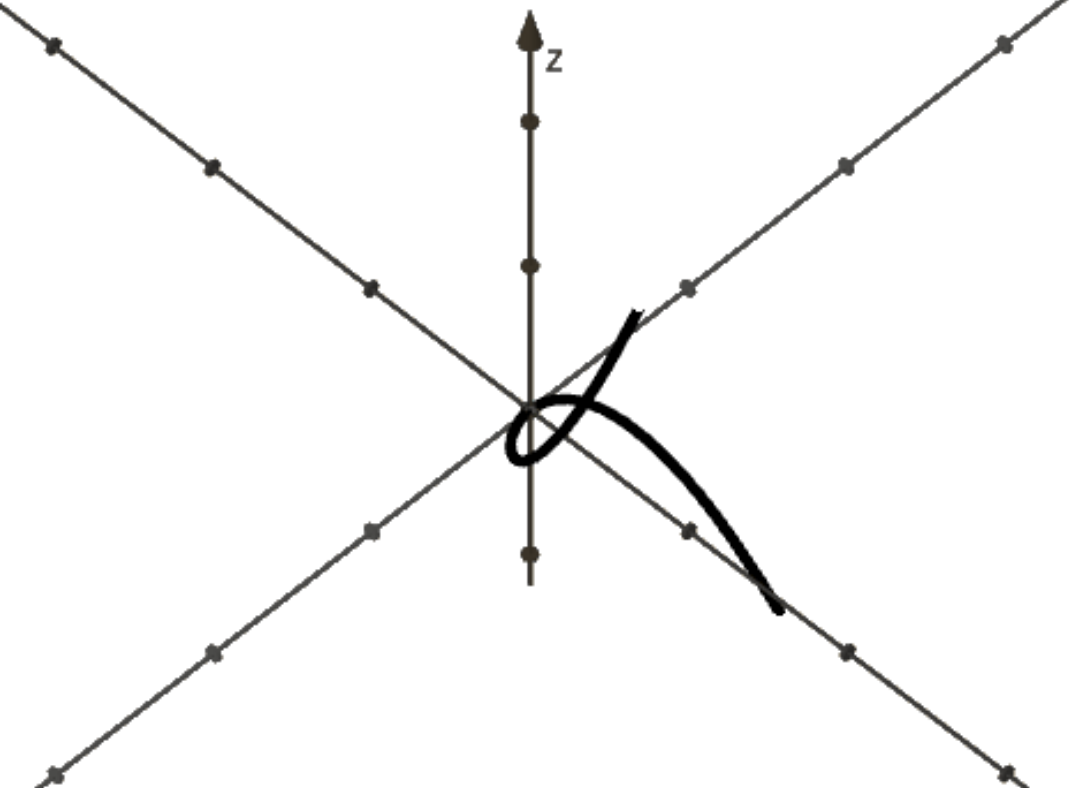
\includegraphics[width=0.3\linewidth]{Imagenes/curva normal}
			\caption{Curva racional en la carta afín $U_0$ dada por $t\mapsto (t,t^2,t^3)$.}
			\label{fig:curva-normal}
		\end{figure}
	
		Por el teorema \ref{encajesubvariedades}, la aplicación $\nu_d=\varphi_{\oo(d)}$ es un encaje holomorfo llamado \textbf{encaje de Veronese}. Por lo tanto, el haz lineal $\oo(d)$ es un haz lineal muy amplio. En particular, el haz lineal $\oo(1)$ es un haz amplio de $\pp^n$. 
	\end{example}